\documentclass[9pt]{report}
% generated by Madoko, version 1.0.3
%mdk-data-line={1}


\usepackage[heading-base={2},section-num={False},bib-label={hide}]{madoko2}


\begin{document}



%mdk-data-line={10}
\pagenumbering{roman}%mdk

%mdk-data-line={13}
\mdxtitleblockstart{}
%mdk-data-line={13}
\mdxtitle{\mdline{13}Copernicus Atmosphere Monitoring Service}%mdk

%mdk-data-line={16}
\mdxsubtitle{\mdline{16}Technical User Guide}%mdk
\mdxauthorstart{}
%mdk-data-line={21}
\mdxauthorname{\mdline{21}Vyron Vasileiadis}%mdk
\mdxauthorend\mdtitleauthorrunning{}{}\mdxtitleblockend%mdk

%mdk-data-line={15}
\begin{abstract}%mdk

%mdk-data-line={16}
\noindent\mdline{16}The abstract.%mdk
%mdk
\end{abstract}%mdk

%mdk-data-line={19}
\noindent\mdline{19}\newpage{}\mdline{19}%mdk
\mdline{21}
\begin{mdtoc}%mdk

\section*{Contents}\label{sec-contents}%mdk%mdk

\begin{mdtocblock}%mdk

\mdtocitemx{sec-introduction}{\mdref{sec-introduction}{1.\hspace*{0.5em}Introduction}}%mdk

\mdtocitemx{sec-study-area-data-materials}{\mdref{sec-study-area-data-materials}{2.\hspace*{0.5em}Study Area, Data \& Materials}}%mdk

\begin{mdtocblock}%mdk

\mdtocitemx{sec-pollutants}{\mdref{sec-pollutants}{2.1.\hspace*{0.5em}Pollutants}}%mdk

\begin{mdtocblock}%mdk

\mdtocitemx{sec-surface-ozone-o3}{\mdref{sec-surface-ozone-o3}{2.1.1.\hspace*{0.5em}Surface Ozone (O\mdsub{3})}}%mdk

\mdtocitemx{sec-nox--nitric-oxide-no-nitrogen-dioxide-no2}{\mdref{sec-nox--nitric-oxide-no-nitrogen-dioxide-no2}{2.1.2.\hspace*{0.5em}NO\mdsub{x}: Nitric Oxide (NO) + Nitrogen Dioxide (NO\mdsub{2})}}%mdk
%mdk
\end{mdtocblock}%mdk

\mdtocitemx{sec-product-services}{\mdref{sec-product-services}{2.2.\hspace*{0.5em}Product Services}}%mdk

\begin{mdtocblock}%mdk

\mdtocitemx{sec-global}{\mdref{sec-global}{2.2.1.\hspace*{0.5em}Global}}%mdk

\mdtocitemx{sec-european-scale}{\mdref{sec-european-scale}{2.2.2.\hspace*{0.5em}European-scale}}%mdk
%mdk
\end{mdtocblock}%mdk

\mdtocitemx{sec-data-access}{\mdref{sec-data-access}{2.3.\hspace*{0.5em}Data access}}%mdk
%mdk
\end{mdtocblock}%mdk

\mdtocitemx{sec-models}{\mdref{sec-models}{3.\hspace*{0.5em}Models}}%mdk

\begin{mdtocblock}%mdk

\mdtocitemx{sec-global}{\mdref{sec-global}{3.1.\hspace*{0.5em}Global}}%mdk

\mdtocitemx{sec-european-scale}{\mdref{sec-european-scale}{3.2.\hspace*{0.5em}European-scale}}%mdk

\begin{mdtocblock}%mdk

\mdtocitemx{sec-chimere}{\mdref{sec-chimere}{3.2.1.\hspace*{0.5em}CHIMERE}}%mdk

\mdtocitemx{sec-emep}{\mdref{sec-emep}{3.2.2.\hspace*{0.5em}EMEP}}%mdk

\mdtocitemx{sec-eurad-im}{\mdref{sec-eurad-im}{3.2.3.\hspace*{0.5em}EURAD-IM}}%mdk

\mdtocitemx{sec-lotos-euros}{\mdref{sec-lotos-euros}{3.2.4.\hspace*{0.5em}LOTOS-EUROS}}%mdk

\mdtocitemx{sec-match}{\mdref{sec-match}{3.2.5.\hspace*{0.5em}MATCH}}%mdk

\mdtocitemx{sec-mocage}{\mdref{sec-mocage}{3.2.6.\hspace*{0.5em}MOCAGE}}%mdk

\mdtocitemx{sec-silam}{\mdref{sec-silam}{3.2.7.\hspace*{0.5em}SILAM}}%mdk

\mdtocitemx{sec-ensemble}{\mdref{sec-ensemble}{3.2.8.\hspace*{0.5em}ENSEMBLE}}%mdk

\mdtocitemx{sec-availability-statistics}{\mdref{sec-availability-statistics}{3.2.9.\hspace*{0.5em}Availability statistics}}%mdk
%mdk
\end{mdtocblock}%mdk
%mdk
\end{mdtocblock}%mdk

\mdtocitemx{sec-results-discussions}{\mdref{sec-results-discussions}{4.\hspace*{0.5em}Results \& Discussions}}%mdk

\mdtocitemx{sec-conclusions}{\mdref{sec-conclusions}{5.\hspace*{0.5em}Conclusions}}%mdk

\mdtocitemx{sec-bibliography}{\mdref{sec-bibliography}{References}}%mdk
%mdk
\end{mdtocblock}%mdk
%mdk
\end{mdtoc}%mdk

%mdk-data-line={23}
\noindent\mdline{23}\newpage{}\mdline{23}%mdk
\mdline{25}
\begin{mdtoc}%mdk

\section*{Figures}\label{sec-figures}%mdk%mdk

\begin{mdtocblock}%mdk

\mdtocitemx{cams-catalogue}{\mdref{cams-catalogue}{\mdcaptionlabel{1}. Available options and details of CAMS Catalogue product ~\emph{Global analyses of chemical species - nitrogen dioxide}}}%mdk

\mdtocitemx{global-map}{\mdref{global-map}{\mdcaptionlabel{2}. Global analysis of NO\mdsub{2} concentration for December 4th, 2016}}%mdk

\mdtocitemx{global-data}{\mdref{global-data}{\mdcaptionlabel{3}. User Interface of ECMWF website for downloading data of global analyses and forecasts.}}%mdk

\mdtocitemx{global-data-additional}{\mdref{global-data-additional}{\mdcaptionlabel{4}. Additional filtering of global analyses' and forecasts' data before downloading.}}%mdk

\mdtocitemx{ensemble-tab}{\mdref{ensemble-tab}{\mdcaptionlabel{5}. Available options in \emph{Ensemble Analysis and Forecast} tab}}%mdk

\mdtocitemx{regional-map-details}{\mdref{regional-map-details}{\mdcaptionlabel{6}. Outline of analyses and forecast maps of regional products.}}%mdk

\mdtocitemx{ensemble-maps}{\mdref{ensemble-maps}{\mdcaptionlabel{7}. Analysis of NO\mdsub{2} concentration on 00:00 UTC December 4th, 2016 issued from the ENSEMBLE model.}}%mdk

\mdtocitemx{regional-maximum}{\mdref{regional-maximum}{\mdcaptionlabel{8}. Maximum concentrations of NO\mdsub{2} on December 4th, 2016 as calculated from all models and their ensemble.}}%mdk

\mdtocitemx{regional-epsgram}{\mdref{regional-epsgram}{\mdcaptionlabel{9}. 4-day forecast of O\mdsub{3}, NO\mdsub{2}, SO\mdsub{2} and PM\mdsub{10} at the city of Athens for the period between December 4th - December 8th, 2016.}}%mdk

\mdtocitemx{chimere-map}{\mdref{chimere-map}{\mdcaptionlabel{10}. Forecast and analysis maps of NO\mdsub{2} concentration for December 4th, 2016 issued by the CHIMERE model.}}%mdk

\begin{mdtocblock}%mdk

\mdtocitemx{}{\mdref{}{(a)  Forecast issued on December 3rd, 2016}}%mdk

\mdtocitemx{}{\mdref{}{(b)  Analysis issued on December 5th, 2016}}%mdk
%mdk
\end{mdtocblock}%mdk
%mdk
\end{mdtocblock}%mdk
%mdk
\end{mdtoc}%mdk

%mdk-data-line={27}
\noindent\mdline{27}\newpage{}\mdline{27}%mdk
\mdline{29}
\begin{mdtoc}%mdk

\section*{Tables}\label{sec-tables}%mdk%mdk

\begin{mdtocblock}%mdk

\mdtocitemx{models-1}{\mdref{models-1}{\mdcaptionlabel{1}. General characteristics of the regional models.}}%mdk

\mdtocitemx{models-2}{\mdref{models-2}{\mdcaptionlabel{2}. Characteristics of the daily assimilation chains of the regional models}}%mdk

\mdtocitemx{chimere-portfolio}{\mdref{chimere-portfolio}{\mdcaptionlabel{3}. Products of CHIMERE model}}%mdk

\mdtocitemx{emep-portfolio}{\mdref{emep-portfolio}{\mdcaptionlabel{4}. Products of EMEP model}}%mdk

\mdtocitemx{eurad-portfolio}{\mdref{eurad-portfolio}{\mdcaptionlabel{5}. Products of EURAD-IM model}}%mdk

\mdtocitemx{lotos-portfolio}{\mdref{lotos-portfolio}{\mdcaptionlabel{6}. Products of LOTOS-EUROS model}}%mdk

\mdtocitemx{match-portfolio}{\mdref{match-portfolio}{\mdcaptionlabel{7}. Products of MATCH model}}%mdk

\mdtocitemx{mocage-portfolio}{\mdref{mocage-portfolio}{\mdcaptionlabel{8}. Products of MOCAGE model}}%mdk

\mdtocitemx{silam-portfolio}{\mdref{silam-portfolio}{\mdcaptionlabel{9}. Products of SILAM model}}%mdk

\mdtocitemx{ensemble-portfolio}{\mdref{ensemble-portfolio}{\mdcaptionlabel{10}. Products of SILAM model}}%mdk

\mdtocitemx{models-3}{\mdref{models-3}{\mdcaptionlabel{11}. Availabilty statistics of models' outputs for usage in ENSEMBLE}}%mdk
%mdk
\end{mdtocblock}%mdk
%mdk
\end{mdtoc}%mdk

%mdk-data-line={31}
\noindent\mdline{31}\newpage{}\mdline{31}%mdk

%mdk-data-line={33}
\pagenumbering{arabic}%mdk

%mdk-data-line={36}
\section{\mdline{36}1.\hspace*{0.5em}\mdline{36}Introduction}\label{sec-introduction}%mdk%mdk

%mdk-data-line={38}
\noindent\mdline{38}The chemical composition of the air close to Earth’s surface, generally referred as \mdline{38}\emph{air quality}\mdline{38} (AQ), directly affects human and animal health and also the vegetation. 
Recently, the World Health Organization reported that in 2012 around 3.7 million deaths were attributable to ambient air pollution\mdline{39} \mdline{39}\mdfootnote{1}{%mdk-data-line={50}
%mdk-data-line={50}
\noindent\mdline{50}http://www.who.int/phe/health\mdline{50}\_\mdline{50}topics/outdoorair/databases/en/%mdk
\label{fn-intro1}%mdk%mdk
}\mdline{39}%mdk

%mdk-data-line={41}
\mdline{41}Since the Helsinki Protocol in 1985, many regions and countries, including the European Union countries, have progressively put in place tools to regulate and to control the emissions of the main air pollutants. 
This has led to an important effort to monitor the air composition near the surface but also to develop air quality forecasting systems in experimental or operational modes (see reviews by Ebel et al., 2005; Menut and Bessagnet, 2010).
These tools can be used in cases of high pollution episodes to inform people and to take emergency measures to prevent harming effects. 
They can also be used for policy makers for the regulations on air pollutant emissions and for monitoring the effect of these regulations on air quality.%mdk

%mdk-data-line={46}
\mdline{46}The Copernicus Atmosphere Monitoring Service (CAMS) 
has been developed to meet these needs, aiming at supporting policymakers, 
business and citizens with enhanced atmospheric environmental information.%mdk

%mdk-data-line={52}
\section{\mdline{52}2.\hspace*{0.5em}\mdline{52}Study Area, Data \mdline{52}\&\mdline{52} Materials}\label{sec-study-area-data-materials}%mdk%mdk

%mdk-data-line={54}
\noindent\mdline{54}\{Introduction\}
Pollutants\mdline{55} \mdline{55}-\mdline{55}\textgreater{}\mdline{55} Areas\mdline{55} \mdline{55}-\mdline{55}\textgreater{}\mdline{55} Services%mdk

%mdk-data-line={57}
\subsection{\mdline{57}2.1.\hspace*{0.5em}\mdline{57}Pollutants}\label{sec-pollutants}%mdk%mdk

%mdk-data-line={59}
\subsubsection{\mdline{59}2.1.1.\hspace*{0.5em}\mdline{59}Surface Ozone (O\mdline{59}\mdsub{3}\mdline{59})}\label{sec-surface-ozone-o3}%mdk%mdk

%mdk-data-line={61}
\noindent\mdline{61}Ozone (O\mdline{61}\mdsub{3}\mdline{61}) in the troposphere (the lowermost part of the atmosphere, from the surface to 6-15 km height depending on the latitude) is highly relevant for the Earth’s climate, ecosystems, and human health.
Tropospheric ozone is the third largest contributor to greenhouse radiative forcing after carbon dioxide and methane\mdline{62}~(Forster et al.,~\mdcite{forster2007changes}{2007})\mdline{62}.
It is part of the Earth’s shield against ultraviolet radiation, particularly when there is stratospheric ozone depletion\mdline{63}~(Sabziparvar et al.,~\mdcite{sabziparvar1998changes}{1998})\mdline{63}.%mdk

%mdk-data-line={65}
\mdline{65}Ozone plays a crucial role in tropospheric chemistry as the main precursor for the OH radical which determines the oxidation capacity of the troposphere\mdline{65}~(Seinfeld and Pandis,~\mdcite{seinfeld2006atmospheric}{2006})\mdline{65}. 
It is a toxic air pollutant affecting human health\mdline{66}~(Bell et al.,~\mdcite{bell2006exposure}{2006})\mdline{66} and agriculture\mdline{66}~(Fowler et al.,~\mdcite{fowler2008ground}{2008})\mdline{66}.
Furthermore, through plant damage, it impedes the uptake of carbon into the biosphere\mdline{67}~(Sitch et al.,~\mdcite{sitch2007indirect}{2007})\mdline{67}.%mdk

%mdk-data-line={69}
\mdline{69}Accurate long-term measurements of ozone in the troposphere, including near the earth surface in unpolluted and polluted environments, are needed in order to assess the impacts of tropospheric ozone on the earth system, human health and ecosystems, and to detect changes in the atmospheric composition which could aggravate or reduce these impacts because of changing ozone precursor emissions or climate change.%mdk

%mdk-data-line={71}
\subsubsection{\mdline{71}2.1.2.\hspace*{0.5em}\mdline{71}NO\mdline{71}\mdsub{x}\mdline{71}: Nitric Oxide (NO)\mdline{71} \mdline{71}+ Nitrogen Dioxide (NO\mdline{71}\mdsub{2}\mdline{71})}\label{sec-nox--nitric-oxide-no-nitrogen-dioxide-no2}%mdk%mdk

%mdk-data-line={73}
\noindent\mdline{73}NO\mdline{73}\mdsub{x}\mdline{73} is a generic term for the mono-nitrogen oxides\mdline{73}~(Mollenhauer and Tschöke,~\mdcite{mollenhauer2010handbook}{2010}; Omidvarborna et al.,~\mdcite{omidvarborna2015113}{2015})\mdline{73}, nitric oxide (NO) and nitrogen dioxide (NO\mdline{73}\mdsub{2}\mdline{73}).
They are produced from the reaction among nitrogen, oxygen and even hydrocarbons (during combustion), especially at high temperatures\mdline{74}~(Omidvarborna et al.,~\mdcite{omidvarborna2015113}{2015}; Annamalai,~\mdcite{annamalai2007combustion}{2007})\mdline{74}.%mdk

%mdk-data-line={76}
\mdline{76}Because NO\mdline{76}\mdsub{x}\mdline{76} are transparent to most wavelengths of light, they allow the vast majority of photons to pass through and, therefore, have a lifetime of at least several days. 
Because NO\mdline{77}\mdsub{2}\mdline{77} is  recycled from NO by the photo reaction of VOC (volatile organic compounds) to make more ozone, NO\mdline{77}\mdsub{2}\mdline{77} seems to have an even longer lifetime and is capable of traveling considerable distances before creating ozone.  Weather systems usually travel over the earth’s surface and allow the atmospheric effects to move downwind for several hundred miles.
This was noted in EPA reports more than twenty years ago.\mdline{78}~(Clean Air Technology Center et al.,~\mdcite{epabulletin}{1999})\mdline{78}
These reports found that each major city on the East coast has a plume of ozone that extends more than a hundred miles out to sea before concentrations drop to 100 parts per billion (ppb).%mdk

%mdk-data-line={81}
\mdline{81}NOx mainly impacts on respiratory conditions causing inflammation of the airways at high levels. Long term exposure can decrease lung function, increase the risk of respiratory conditions and increases the response to allergens. 
NO\mdline{82}\mdsub{x}\mdline{82} also contributes to the formation of fine particles\mdline{82}\mdfootnote{2}{%mdk-data-line={84}
%mdk-data-line={84}
\noindent\mdline{84}http://www.icopal-noxite.co.uk/nox-problem/nox-pollution.aspx\mdline{84}\#\mdline{84}sthash.esEBqdj6.dpuf%mdk
\label{fn-nox-1}%mdk%mdk
}\mdline{82}.%mdk

%mdk-data-line={85}
\subsection{\mdline{85}2.2.\hspace*{0.5em}\mdline{85}Product Services}\label{sec-product-services}%mdk%mdk

%mdk-data-line={87}
\noindent\mdline{87}\emph{an intro here}\mdline{87}%mdk

%mdk-data-line={89}
\subsubsection{\mdline{89}2.2.1.\hspace*{0.5em}\mdline{89}Global}\label{sec-global}%mdk%mdk

%mdk-data-line={90}
\noindent\mdline{90}The global products are provided by the ECMWF Composition-Integrated Forecast System (C-IFS).
The services consist of daily near real-time analyses and forecasts up to five days, and a re-analysis, currently for the period 2003\mdline{91} \mdline{91}- 2012. 
The geographical area covered is the whole Earth, from 180\mdline{92}\textdegree{}\mdline{92}W to 180\mdline{92}\textdegree{}\mdline{92} and 90\mdline{92}\textdegree{}\mdline{92}S to 90\mdline{92}\textdegree{}\mdline{92}N. 
Vertically global services cover both the troposphere and stratosphere.%mdk

%mdk-data-line={95}
\paragraph{\mdline{95}Global analyses of chemical species}\label{sec-global-analyses-of-chemical-species}%mdk%mdk

%mdk-data-line={96}
\noindent\mdline{96}\mdbr
\mdline{97}This service provides daily analyses of chemical species, including O\mdline{97}\mdsub{3}\mdline{97}, NO and NO\mdline{97}\mdsub{2}\mdline{97}. 
The Service became operational on July 1st 2015 and provides data every 6 hours.%mdk

%mdk-data-line={100}
\paragraph{\mdline{100}Global forecasts of chemical species}\label{sec-global-forecasts-of-chemical-species}%mdk%mdk

%mdk-data-line={101}
\noindent\mdline{101}\mdbr
\mdline{102}This service provides daily forecasts up to 5 days of chemical species, including O\mdline{102}\mdsub{3}\mdline{102}, NO and NO\mdline{102}\mdsub{2}\mdline{102}. 
The service became operational on July 1st 2015.%mdk

%mdk-data-line={105}
\paragraph{\mdline{105}MACC global reanalysis of assimilated chemical species}\label{sec-macc-global-reanalysis-of-assimilated-chemical-species}%mdk%mdk

%mdk-data-line={106}
\noindent\mdline{106}\mdbr
\mdline{107}This service provides global reanalysis of chemical species that are directly constrained by observations.
Only O\mdline{108}\mdsub{3}\mdline{108} and NO\mdline{108}\mdsub{2}\mdline{108} reanalysis data are available. 
This service time coverage spans from January 2003 to 31 December 2012, and has a time resolution of 3 hours.
Horizontal resolution is approximately 60 km.%mdk

%mdk-data-line={112}
\paragraph{\mdline{112}MACC global reanalysis of non-assimilated chemical species}\label{sec-macc-global-reanalysis-of-non-assimilated-chemical-species}%mdk%mdk

%mdk-data-line={113}
\noindent\mdline{113}\mdbr
\mdline{114}This service provides global reanalysis of chemical species that are not directly constrained by observations. 
Only NO and NO\mdline{115}\mdsub{2}\mdline{115} reanalysis data are available. 
This service time coverage spans from January 2003 to 31 December 2012, and has a time resolution of 3 hours.
Horizontal resolution is 1.125\mdline{117}\textdegree{}\mdline{117} x 1.125\mdline{117}\textdegree{}\mdline{117}.%mdk

%mdk-data-line={119}
\subsubsection{\mdline{119}2.2.2.\hspace*{0.5em}\mdline{119}European-scale}\label{sec-european-scale}%mdk%mdk

%mdk-data-line={120}
\noindent\mdline{120}The European-scale regional products are provided for the European domain (25\mdline{120}\textdegree{}\mdline{120}W to 45\mdline{120}\textdegree{}\mdline{120}E and from 30\mdline{120}\textdegree{}\mdline{120}N to 70\mdline{120}\textdegree{}\mdline{120}N). 
The service provides daily 4-day forecasts of the main air quality species, including O\mdline{121}\mdsub{3}\mdline{121}, NO, NO\mdline{121}\mdsub{2}\mdline{121}, and analyses of the day before, from 7 state-of-the-art atmospheric chemistry models and from the median ensemble calculated from the 7 model forecasts. 
The 7 atmospheric chemistry models are: CHIMERE, EMEP, EURAD-IM, LOTOS-EUROS, MATCH, MOCAGE, SILAM.
The regional service also provides daily posteriori interim re-analyses based on fast-track in-situ observations, and annual re-analyses based on fully validated in-situ observations.%mdk

%mdk-data-line={125}
\paragraph{\mdline{125}European-scale air quality analysis}\label{sec-european-scale-air-quality-analysis}%mdk%mdk

%mdk-data-line={126}
\noindent\mdline{126}\mdbr
\mdline{127}This service provides European-scale air quality analyses for every hour of the previous day for every of the 7 models and the ensemble median. 
The service became operational on October 1st 2015.%mdk

%mdk-data-line={130}
\paragraph{\mdline{130}European-scale air quality forecast}\label{sec-european-scale-air-quality-forecast}%mdk%mdk

%mdk-data-line={131}
\noindent\mdline{131}\mdbr
\mdline{132}This service provides European-scale air quality forecasts for every hour up to 4 days in advance for every of the 7 models and the ensemble median. 
The service became operational on October 1st 2015.%mdk

%mdk-data-line={135}
\subsection{\mdline{135}2.3.\hspace*{0.5em}\mdline{135}Data access}\label{sec-data-access}%mdk%mdk

%mdk-data-line={136}
\noindent\mdline{136}Products delivered by CAMS are provided free of charge, since October 1st 2015.
There is a universal search engine available on the CAMS web portal. 
The default procedure that should be used by common user is the following:%mdk

%mdk-data-line={140}
\begin{enumerate}[noitemsep,topsep=\mdcompacttopsep]%mdk

%mdk-data-line={140}
\item\mdline{140}Go to the CAMS website http://atmosphere.copernicus.eu%mdk

%mdk-data-line={141}
\item\mdline{141}Click CATALOGUE. The CAMS catalogue lists the various CAMS products.%mdk

%mdk-data-line={142}
\item\mdline{142}Filter the catalogue for the service or product of interest. The filters change depending on the selection.%mdk

%mdk-data-line={143}
\item\mdline{143}Once a suitable product is identified, click on its name. A popup window opens, showing details and a preview.%mdk

%mdk-data-line={144}
\item\mdline{144}At the bottom of the window follow the links to Plots (maps and graphs), Data Access, Documentation, etc. These links take you to pages specific to the selected product.%mdk

%mdk-data-line={145}
\item\mdline{145}From here the procedure is different for every product, depending on the provider.%mdk
%mdk
\end{enumerate}%mdk

%mdk-data-line={147}
\noindent\mdline{147}In particular:
\mdline{148}\mdbr
\mdline{149}\mdbr
\mdline{150}\textbf{Global products}\mdline{150} are served by European Centre for Medium-Range Weather Forecasts (ECMWF).
A registration is required to access the data. 
CAMS provides its global data sets in two different ways.%mdk

%mdk-data-line={154}
\mdline{154}One option is the interactive web interface of ECMWF\mdline{154}\mdfootnote{3}{%mdk-data-line={161}
%mdk-data-line={161}
\noindent\mdline{161}http://apps.ecmwf.int/datasets/data/cams-nrealtime/levtype=sfc/%mdk
\label{fn-ecmwf-web}%mdk%mdk
}\mdline{154} data server which provides batch data access to real-time analyses and forecasts, reanalysis results in GRIB and NetCDF format.
It also provides a programmatic way of accessing data using python language. Detailed information can be found in ECMWF wiki\mdline{155}\mdfootnote{4}{%mdk-data-line={162}
%mdk-data-line={162}
\noindent\mdline{162}https://software.ecmwf.int/wiki/display/WEBAPI/Access+ECMWF+Public+Datasets%mdk
\label{fn-ecmwf-wiki}%mdk%mdk
}\mdline{155}.%mdk

%mdk-data-line={157}
\mdline{157}The second option is through the ECMWF FTP server\mdline{157}\mdfootnote{5}{%mdk-data-line={163}
%mdk-data-line={163}
\noindent\mdline{163}ftp://dissemination.ecmwf.int/%mdk
\label{fn-ecmwf-ftp}%mdk%mdk
}\mdline{157}, which provides archived real-time forecasts of the latest three days in GRIB and NetCDF format.
CAMS data files can be accessed through directory \mdline{158}~\mdline{158}\mdcode{/DATA/CAMS\_NREALTIME/\$\{YYYYMMDDhh\}}\mdline{158} and follow a naming convention proposed by World Meteorological Organization (WMO). 
Detailed information can be found in CAMS website\mdline{159}\mdfootnote{6}{%mdk-data-line={164}
%mdk-data-line={164}
\noindent\mdline{164}http://atmosphere.copernicus.eu/ftp-access-global-data%mdk
\label{fn-ftp}%mdk%mdk
}\mdline{159}.%mdk

%mdk-data-line={166}
\mdline{166}\mdbr
\mdline{167}\textbf{European-scale products}\mdline{167} are accessed directly through CAMS web portal\mdline{167}\mdfootnote{7}{%mdk-data-line={186}
%mdk-data-line={186}
\noindent\mdline{186}http://www.regional.atmosphere.copernicus.eu/index.php?category=data\mdline{186}\_\mdline{186}access\mdline{186}\&\mdline{186}subensemble=dataserver\mdline{186}\_\mdline{186}services%mdk
\label{fn-regional-web}%mdk%mdk
}\mdline{167}. Files are available in Grib2 format and Netcdf format for model ENSEMBLE for both Forecast (surface as well as other levels ) \mdline{167}\&\mdline{167} Analysis (surface).
Files are available only in Netcdf format for models: CHIMERE, EMEP, EURAD, LOTOSEUROS, MATCH, MOCAGE, SILAM for both Forecast (surface as well as other levels) \mdline{168}\&\mdline{168} Analysis (surface). 
There are six available choices:%mdk

%mdk-data-line={171}
\begin{itemize}[noitemsep,topsep=\mdcompacttopsep]%mdk

%mdk-data-line={171}
\item\mdline{171}\textbf{Download online data}\mdline{171}\mdbr
\mdline{172}Files produced less than 30 days ago are available. Available formats are GRIB2, NetCDF or TXT, depending on the type of product.%mdk

%mdk-data-line={173}
\item\mdline{173}\textbf{Download archived data}\mdline{173}\mdbr
\mdline{174}Archived data are older than 30 days. Archiving starts in October 2015. Available formats are GRIB2, NetCDF or TXT, depending on the type of product.%mdk

%mdk-data-line={175}
\item\mdline{175}\textbf{Download reanalysis data}\mdline{175}\mdbr
\mdline{176}Download numerical data about atmospheric composition in Europe (reanalysis). Archiving starts in 2015 and the available data format is NetCDF.%mdk

%mdk-data-line={177}
\item\mdline{177}\textbf{Download on map viewing}\mdline{177}\mdbr
\mdline{178}Visualize data over a map of Europe. Very useful for an interesting air quality phenomenon spotted on a map view.%mdk

%mdk-data-line={179}
\item\mdline{179}\textbf{Data server - subscribe mode}\mdline{179}\mdbr
\mdline{180}Data server subsribe mode allows users to subscribe to a product, to choose the delivery type (ftp,\mdline{180}\dots{}\mdline{180}), as well as the delivery time (upon arrival, on a specific chosen time).%mdk

%mdk-data-line={181}
\item\mdline{181}\textbf{Data server - catalogue}\mdline{181}\mdbr
\mdline{182}Consult the catalogue of metadata, in order to discover all the CAMS Regional Air Quality products.%mdk
%mdk
\end{itemize}%mdk

%mdk-data-line={188}
\section{\mdline{188}3.\hspace*{0.5em}\mdline{188}Models}\label{sec-models}%mdk%mdk

%mdk-data-line={190}
\subsection{\mdline{190}3.1.\hspace*{0.5em}\mdline{190}Global}\label{sec-global}%mdk%mdk

%mdk-data-line={191}
\noindent\mdline{191}The operational CAMS global assimilation and forecasting system uses fully integrated chemistry in the ECMWF Integrated Forecasting System (IFS). The version of the IFS is named Composition-IFS (C-IFS). 
C-IFS makes it possible\mdline{192} \mdline{192}%mdk

%mdk-data-line={194}
\begin{itemize}%mdk

%mdk-data-line={194}
\item{}
%mdk-data-line={194}
\mdline{194}to use the detailed meteorological simulation of the IFS for the simulation of the fate of constituents,\mdline{194} \mdline{194}%mdk%mdk

%mdk-data-line={196}
\item{}
%mdk-data-line={196}
\mdline{196}to simulate atmospheric chemistry globally at high resolution because of the computational parallel efficiency of the IFS,\mdline{196} \mdline{196}%mdk%mdk

%mdk-data-line={198}
\item{}
%mdk-data-line={198}
\mdline{198}to use the IFS data assimilation system to assimilate observation of atmospheric composition and\mdline{198} \mdline{198}%mdk%mdk

%mdk-data-line={200}
\item{}
%mdk-data-line={200}
\mdline{200}to simulate feedback between atmospheric composition and weather. Different chemical schemes can be used with the current operational version being based on the CB05 scheme.%mdk%mdk
%mdk
\end{itemize}%mdk

%mdk-data-line={202}
\noindent\mdline{202}C-IFS  replaces the coupled system IFS-MOZART for forecast and assimilation of reactive gases within the pre-operational Copernicus Atmosphere Monitoring Service.%mdk

%mdk-data-line={204}
\subsection{\mdline{204}3.2.\hspace*{0.5em}\mdline{204}European-scale}\label{sec-european-scale}%mdk%mdk

%mdk-data-line={206}
\noindent\mdline{206}Each of the seven models is run at its own horizontal and vertical resolutions, with the horizontal resolutions varying between 10 and 20 km. 
This range of resolutions is not designed to reproduce local aspects of air pollution but to provide concentrations of pollutants at the regional scale that can then be used in particular as boundary conditions for air quality forecasts at finer resolution.%mdk

%mdk-data-line={209}
\mdline{209}The range of the forecasts is 96h from 00:00 UTC on Day0 with hourly outputs on eight vertical levels (surface, 50, 250, 500, 1000, 2000, 3000 and 5000m). 
Day0 is defined as the day when the forecast is run. 
The forecast initial time/date is Day0 at 00:00 UTC and final time/date is Day3 at 24:00UTC. 
For each time step (1h), the individual model fields are interpolated on these vertical levels and on the same regular 0.1\mdline{212}\textdegree{}\mdline{212} latitude by 0.1\mdline{212}\textdegree{}\mdline{212} longitude grid over the European domain. 
It is from these re-gridded fields that the ensemble median and verification products are calculated.%mdk

%mdk-data-line={215}
\mdline{215}The analysis at the surface for Day0–1 (the day before Day0) is run daily a posteriori on Day0 using the assimilation of the hourly data from the AQ monitoring stations available in Europe between 00:00 and 23:00UTC on Day0– 1. 
Like for the forecasts, Day0 is defined as the day when the analysis is run. 
The analysis initial time/date is Day0–1 at 00:00 UTC and final time/date is Day0–1 at 23:00 UTC. 
Similarly to the forecasts, the hourly individual model fields are interpolated on the same 0.1\mdline{218}\textdegree{}\mdline{218} latitude by 0.1\mdline{218}\textdegree{}\mdline{218} longitude grid. 
The analyses are only produced at the surface level.%mdk

%mdk-data-line={221}
\mdline{221}An overview of the characteristics of the seven models can be seen in tables\mdline{221}~\mdref{models-1}{\mdcaptionlabel{1}}\mdline{221} and\mdline{221}~\mdref{models-2}{\mdcaptionlabel{2}}\mdline{221}.
Detailed descriptions of each model are presented in the following sections.%mdk

%mdk-data-line={224}
\begin{table}[h!]%mdk
\begin{mdcenter}%mdk
{\mdlineheight{1.5em}{\mdfontsize{8pt}\begin{mdtabular}{4}{\dimeval{(\linewidth)/4}}{1ex}%mdk
\begin{tabular}{llll}{\bfseries\mdline{225}\textbf{Model}\mdline{225}}&{\bfseries\mdline{225}\textbf{Operated By}\mdline{225}}&{\bfseries\mdline{225}\textbf{Horizontal Resolution}\mdline{225}}&{\bfseries\mdline{225}\textbf{Vertical Resolution}\mdline{225}}\\

\midrule
\mdline{227}CHIMERE&\mdline{227}INERIS, France&\mdline{227} 0.1\mdline{227}\textdegree{}\mdline{227}×0.1\mdline{227}\textdegree{}\mdline{227}&\mdline{227}8 levels\\
\mdline{228}&\mdline{228}&\mdline{228}&\mdline{228}Top at 500 hPa\\
\mdline{229}EMEP&\mdline{229}MET Norway, Norway&\mdline{229}0.25\mdline{229}\textdegree{}\mdline{229}x1.25\mdline{229}\textdegree{}\mdline{229}&\mdline{229}20 levels\\
\mdline{230}&\mdline{230}&\mdline{230}&\mdline{230}Top at 100 hPa\\
\mdline{231}EURAD-IM&\mdline{231}RIU UK, Germany&\mdline{231}15km on a Lambert&\mdline{231}23 levels\\
\mdline{232}&\mdline{232}&\mdline{232}conformal projection&\mdline{232}Top at 100 hPa\\
\mdline{233}LOTOS-EURO&\mdline{233}KNMI, Netherlands&\mdline{233}0.25\mdline{233}\textdegree{}\mdline{233}x1.25\mdline{233}\textdegree{}\mdline{233}&\mdline{233}4 levels\\
\mdline{234}&\mdline{234}&\mdline{234}&\mdline{234}Top at 3.5 km\\
\mdline{235}MATCH&\mdline{235}SMHI, Sweden&\mdline{235}0.2\mdline{235}\textdegree{}\mdline{235}x0.2\mdline{235}\textdegree{}\mdline{235}&\mdline{235}52 levels\\
\mdline{236}&\mdline{236}&\mdline{236}&\mdline{236}Top at 300 hPa\\
\mdline{237}MOCAGE&\mdline{237}Météo-France, France&\mdline{237}0.2\mdline{237}\textdegree{}\mdline{237}x0.2\mdline{237}\textdegree{}\mdline{237}&\mdline{237}47 levels\\
\mdline{238}&\mdline{238}&\mdline{238}&\mdline{238}Top at 5 hPa\\
\mdline{239}SILAM&\mdline{239}FMI, Finland&\mdline{239}0.15\mdline{239}\textdegree{}\mdline{239}x0.15\mdline{239}\textdegree{}\mdline{239}&\mdline{239}8 levels\\
\mdline{240}&\mdline{240}&\mdline{240}&\mdline{240}Top at 6.7 km\\
\end{tabular}\end{mdtabular}

%mdk-data-line={241}
\mdhr{}%mdk

%mdk-data-line={242}
\noindent\mdline{242}\mdcaption{\textbf{Table~\mdcaptionlabel{1}.}~\mdcaptiontext{General characteristics of the regional models.}}%mdk
}}%mdk
\end{mdcenter}\label{models-1}%mdk
%mdk
\end{table}%mdk

%mdk-data-line={243}
\begin{table}[h!]%mdk
\begin{mdbmarginx}{}{}{}{\dimpx{-50}}%mdk
\begin{mdcenter}%mdk
{\mdlineheight{1.5em}{\mdfontsize{8pt}\begin{mdtabular}{4}{\dimeval{(\linewidth)/4}}{1ex}%mdk
\begin{tabular}{llll}{\bfseries\mdline{244}\textbf{Model}\mdline{244}}&{\bfseries\mdline{244}\textbf{Assimilation Method}\mdline{244}}&{\bfseries\mdline{244}\textbf{Observation assimilated}\mdline{244}}&{\bfseries\mdline{244}\textbf{Pollutants analysed}\mdline{244}}\\

\midrule
\mdline{246}CHIMERE&\mdline{246}Optimal interpolation&\mdline{246}O\mdline{246}\mdsub{3}\mdline{246} from surface stations&\mdline{246}O\mdline{246}\mdsub{3}\mdline{246}, NO, NO\mdline{246}\mdsub{2}\mdline{246}\\
\mdline{247}EMEP&\mdline{247}3DVar&\mdline{247}NO\mdline{247}\mdsub{2}\mdline{247} columns from OMI&\mdline{247}O\mdline{247}\mdsub{3}\mdline{247}, NO, NO\mdline{247}\mdsub{2}\mdline{247}\\
\mdline{248}&\mdline{248}&\mdline{248}NO\mdline{248}\mdsub{2}\mdline{248} from surface stations&\mdline{248}O\mdline{248}\mdsub{3}\mdline{248}, NO, NO\mdline{248}\mdsub{2}\mdline{248}\\
\mdline{249}EURAD-IM&\mdline{249}3DVar&\mdline{249}O\mdline{249}\mdsub{3}\mdline{249}, NO, NO\mdline{249}\mdsub{2}\mdline{249} from surface stations&\mdline{249}O\mdline{249}\mdsub{3}\mdline{249}, NO, NO\mdline{249}\mdsub{2}\mdline{249}\\
\mdline{250}&\mdline{250}&\mdline{250}NO\mdline{250}\mdsub{2}\mdline{250} columns from OMI and GOME-2&\mdline{250}O\mdline{250}\mdsub{3}\mdline{250}, NO, NO\mdline{250}\mdsub{2}\mdline{250}\\
\mdline{251}LOTOS-EURO&\mdline{251}Ensemble Kalman filter&\mdline{251}O\mdline{251}\mdsub{3}\mdline{251} from surface stations&\mdline{251}O\mdline{251}\mdsub{3}\mdline{251}, NO, NO\mdline{251}\mdsub{2}\mdline{251}\\
\mdline{252}MATCH&\mdline{252}3DVar&\mdline{252}O\mdline{252}\textasciitilde{}\mdline{252}3, NO\mdline{252}\mdsub{2}\mdline{252} from surface stations&\mdline{252}O\mdline{252}\mdsub{3}\mdline{252}, NO, NO\mdline{252}\mdsub{2}\mdline{252}\\
\mdline{253}MOCAGE&\mdline{253}3DVar&\mdline{253}O\mdline{253}\mdsub{3}\mdline{253} from surface stations&\mdline{253}O\mdline{253}\mdsub{3}\mdline{253}, NO, NO\mdline{253}\mdsub{2}\mdline{253}\\
\mdline{254}SILAM&\mdline{254}4DVar&\mdline{254}O\mdline{254}\textasciitilde{}\mdline{254}3, NO\mdline{254}\mdsub{2}\mdline{254} from surface stations&\mdline{254}O\mdline{254}\mdsub{3}\mdline{254}, NO, NO\mdline{254}\mdsub{2}\mdline{254}\\
\end{tabular}\end{mdtabular}

%mdk-data-line={255}
\mdhr{}%mdk

%mdk-data-line={256}
\noindent\mdline{256}\mdcaption{\textbf{Table~\mdcaptionlabel{2}.}~\mdcaptiontext{Characteristics of the daily assimilation chains of the regional models}}%mdk
}}%mdk
\end{mdcenter}\label{models-2}%mdk%mdk
\end{mdbmarginx}%mdk
\end{table}%mdk

%mdk-data-line={257}
\subsubsection{\mdline{257}3.2.1.\hspace*{0.5em}\mdline{257}CHIMERE}\label{sec-chimere}%mdk%mdk

%mdk-data-line={259}
\noindent\mdline{259}CHIMERE is an Eulerian chemistry-transport model able to simulate concentration fields of gaseous and aerosols species at a regional scale\mdline{259}~(Menut et al.,~\mdcite{menut2013chimere}{2013})\mdline{259}. 
The model is developed under the General Public License licence\mdline{260}\mdfootnote{8}{%mdk-data-line={262}
%mdk-data-line={262}
\noindent\mdline{262}Official website: http://www.lmd.polytechnique.fr/chimere/%mdk
\label{fn-fn}%mdk%mdk
}\mdline{260}. CHIMERE is used for analysis of pollution events, process studies\mdline{260}~(Beekmann and Vautard,~\mdcite{beekmann2010modelling}{2010})\mdline{260}, experimental and operational forecasts\mdline{260}~(Rouil et al.,~\mdcite{rouil2009prev}{2009})\mdline{260}, regional climate studies and trends\mdline{260}~(Colette et al.,~\mdcite{colette2011air}{2011})\mdline{260}, among others.%mdk

%mdk-data-line={264}
\mdline{264}CHIMERE runs over a range of spatial scale from the regional scale (several thousand kilometres) to the urban scale (100-200 Km) with resolutions from 1-2 Km to 100 Km. 
The model runs over the GEMS-MACC domain with a 0.1\mdline{265}\textdegree{}\mdline{265} resolution and 8 vertical levels extending from the surface up to 500 hPa, covering the whole troposhphere.%mdk

%mdk-data-line={267}
\mdline{267}CHIMERE reproduces nicely the day to day O\mdline{267}\mdsub{3}\mdline{267} variation similarly at urban and rural sites with an overestimation which is higher during the winter at urban sites. 
CHIMERE reproduces the daily NO\mdline{268}\mdsub{x}\mdline{268} variability along the year but underestimates significantly the concentration especially during the cold season.%mdk

%mdk-data-line={270}
\mdline{270}Availability information of CHIMERE products as of May 2016 are presented in Table\mdline{270}~\mdref{chimere-portfolio}{\mdcaptionlabel{3}}\mdline{270}.%mdk

%mdk-data-line={272}
\begin{table}[h!]%mdk
\begin{mdcenter}%mdk
{\mdlineheight{1.5em}{\mdfontsize{8pt}\begin{mdtabular}{3}{\dimeval{(\linewidth)/3}}{1ex}%mdk
\begin{tabular}{lll}{\bfseries\mdline{273}}&{\bfseries\mdline{273}\textbf{Forecast}\mdline{273}}&{\bfseries\mdline{273}\textbf{Analysis}\mdline{273}}\\

\midrule
\mdline{275}\textbf{Altitudes}\mdline{275}&\mdline{275}Surface, 50m, 250m, 500m,&\mdline{275}Surface\\
\mdline{276}&\mdline{276}1000m, 2000m, 3000, 5000m&\mdline{276}\\
\mdline{277}\textbf{Available at}&\mdline{277}6:00 UTC&\mdline{277}09:45 UTC for the day before\\
\mdline{278}\textbf{Pollutants}\mdline{278}&\mdline{278}O\mdline{278}\mdsub{3}\mdline{278}, NO, NO\mdline{278}\mdsub{2}\mdline{278}&\mdline{278}O\mdline{278}\mdsub{3}\mdline{278}, NO\mdline{278}*\mdline{278}, NO\mdline{278}\mdsub{2}\mdline{278}\\
\mdline{279}\textbf{Timespan}\mdline{279}&\mdline{279}0-96h, hourly&\mdline{279}0-24h for the day before, hourly\\
\end{tabular}\end{mdtabular}

%mdk-data-line={280}
\noindent\mdline{280}*\mdline{280} Not assimilated%mdk

%mdk-data-line={281}
\mdhr{}%mdk

%mdk-data-line={282}
\noindent\mdline{282}\mdcaption{\textbf{Table~\mdcaptionlabel{3}.}~\mdcaptiontext{Products of CHIMERE model}}%mdk
}}%mdk
\end{mdcenter}\label{chimere-portfolio}%mdk
%mdk
\end{table}%mdk

%mdk-data-line={283}
\subsubsection{\mdline{283}3.2.2.\hspace*{0.5em}\mdline{283}EMEP}\label{sec-emep}%mdk%mdk

%mdk-data-line={284}
\noindent\mdline{284}The EMEP/MSC-W model has been developed at the EMEP Meteorological Synthesizing Centre-West at the Norwegian Meteorological Institute. 
The model has been publicly available as open-source code since 2008, and a detailed description is given in Simpson et al. (2012).%mdk

%mdk-data-line={287}
\mdline{287}One strength of the EMEP model is that its domain extends throughout the whole troposphere, thus taking accurate account of long-range transport of pollutants in the free troposphere. 
As the model is designed mainly for background concentrations, urban increments have not been implemented as in some other models with equally coarse resolution, leading to somewhat lower performance in urban and sub-urban areas. 
However, being one of the main research tools under the UN LRTAP (Long-range Transboundary Air Pollution) convention, the EMEP model is evaluated continuously against measurements of a large range of chemical parameters (including air concentrations, depositions, and trends) ensuring modelling capability with very good overall performance\mdline{289}~(Jonson et al.,~\mdcite{jonson2006first}{2006}; Fagerli and Aas,~\mdcite{fagerli2008trends}{2008}; Genberg et al.,~\mdcite{genberg2013light}{2013})\mdline{289}.%mdk

%mdk-data-line={291}
\mdline{291}Availability information of EMEP products as of May 2016 are presented in Table\mdline{291}~\mdref{emep-portfolio}{\mdcaptionlabel{4}}\mdline{291}.%mdk

%mdk-data-line={293}
\begin{table}[h!]%mdk
\begin{mdcenter}%mdk
{\mdlineheight{1.5em}{\mdfontsize{8pt}\begin{mdtabular}{3}{\dimeval{(\linewidth)/3}}{1ex}%mdk
\begin{tabular}{lll}{\bfseries\mdline{294}}&{\bfseries\mdline{294}\textbf{Forecast}\mdline{294}}&{\bfseries\mdline{294}\textbf{Analysis}\mdline{294}}\\

\midrule
\mdline{296}\textbf{Altitudes}\mdline{296}&\mdline{296}Surface, 50m, 250m, 500m,&\mdline{296}Surface\\
\mdline{297}&\mdline{297}1000m, 2000m, 3000, 5000m&\mdline{297}\\
\mdline{298}\textbf{Available at}&\mdline{298}2:00 UTC&\mdline{298}08:45 UTC for the day before\\
\mdline{299}\textbf{Pollutants}\mdline{299}&\mdline{299}O\mdline{299}\mdsub{3}\mdline{299}, NO, NO\mdline{299}\mdsub{2}\mdline{299}&\mdline{299}O\mdline{299}\mdsub{3}\mdline{299}, NO\mdline{299}*\mdline{299}, NO\mdline{299}\mdsub{2}\mdline{299}\\
\mdline{300}\textbf{Timespan}\mdline{300}&\mdline{300}0-96h, hourly&\mdline{300}0-24h for the day before, hourly\\
\end{tabular}\end{mdtabular}

%mdk-data-line={301}
\noindent\mdline{301}*\mdline{301} Not assimilated%mdk

%mdk-data-line={302}
\mdhr{}%mdk

%mdk-data-line={303}
\noindent\mdline{303}\mdcaption{\textbf{Table~\mdcaptionlabel{4}.}~\mdcaptiontext{Products of EMEP model}}%mdk
}}%mdk
\end{mdcenter}\label{emep-portfolio}%mdk
%mdk
\end{table}%mdk

%mdk-data-line={304}
\subsubsection{\mdline{304}3.2.3.\hspace*{0.5em}\mdline{304}EURAD-IM}\label{sec-eurad-im}%mdk%mdk

%mdk-data-line={305}
\noindent\mdline{305}EURAD-IM is an Eulerian meso-scale chemistry transport model involving advection, diffusion, chemical transformation, wet and dry deposition and sedimentation of tropospheric trace gases and aerosols (Hass et al., 1995, Memmesheimer et al., 2004). It includes 3DVar and 4DVar chemical data assimilation (Elbern et al., 2007) and is able to run in nesting mode.
EURAD-IM has been applied on several recent air pollution studies\mdline{306}~(Monteiro et al.,~\mdcite{monteiro2013bias}{2013}; Paschalidi,~\mdcite{paschalidi2015inverse}{2015})\mdline{306}.%mdk

%mdk-data-line={308}
\mdline{308}Availability information of EURAD-IM products as of May 2016 are presented in Table\mdline{308}~\mdref{eurad-portfolio}{\mdcaptionlabel{5}}\mdline{308}.%mdk

%mdk-data-line={310}
\begin{table}[h!]%mdk
\begin{mdcenter}%mdk
{\mdlineheight{1.5em}{\mdfontsize{8pt}\begin{mdtabular}{3}{\dimeval{(\linewidth)/3}}{1ex}%mdk
\begin{tabular}{lll}{\bfseries\mdline{311}}&{\bfseries\mdline{311}\textbf{Forecast}\mdline{311}}&{\bfseries\mdline{311}\textbf{Analysis}\mdline{311}}\\

\midrule
\mdline{313}\textbf{Altitudes}\mdline{313}&\mdline{313}Surface, 50m, 250m, 500m,&\mdline{313}Surface\\
\mdline{314}&\mdline{314}1000m, 2000m, 3000, 5000m&\mdline{314}\\
\mdline{315}\textbf{Available at}&\mdline{315}6:00 UTC&\mdline{315}09:45 UTC for the day before\\
\mdline{316}\textbf{Pollutants}\mdline{316}&\mdline{316}O\mdline{316}\mdsub{3}\mdline{316}, NO, NO\mdline{316}\mdsub{2}\mdline{316}&\mdline{316}O\mdline{316}\mdsub{3}\mdline{316}, NO\mdline{316}*\mdline{316}, NO\mdline{316}\mdsub{2}\mdline{316}\\
\mdline{317}\textbf{Timespan}\mdline{317}&\mdline{317}0-96h, hourly&\mdline{317}0-24h for the day before, hourly\\
\end{tabular}\end{mdtabular}

%mdk-data-line={318}
\noindent\mdline{318}*\mdline{318} Until April 20th, 2016 NO observations from the German Umweltbundesamt (UBA) were assimilated. Thereafter surface in situ observations from UBA have been removed from the EURAD-IM assimilation chain, to be compliant with CAMS requirements.%mdk

%mdk-data-line={319}
\mdhr{}%mdk

%mdk-data-line={320}
\noindent\mdline{320}\mdcaption{\textbf{Table~\mdcaptionlabel{5}.}~\mdcaptiontext{Products of EURAD-IM model}}%mdk
}}%mdk
\end{mdcenter}\label{eurad-portfolio}%mdk
%mdk
\end{table}%mdk

%mdk-data-line={321}
\subsubsection{\mdline{321}3.2.4.\hspace*{0.5em}\mdline{321}LOTOS-EUROS}\label{sec-lotos-euros}%mdk%mdk

%mdk-data-line={322}
\noindent\mdline{322}The 3-D chemistry-transport model LOTOS-EUROS\mdline{322}~(Schaap et al.,~\mdcite{schaap2008lotos}{2008})\mdline{322} is developed by the Dutch institutes TNO, RIVM and, more recently, KNMI.
It is used for regional-scale air quality forecasts in Europe and the Netherlands\mdline{323}~(Wildt et al.,~\mdcite{de2011six}{2011})\mdline{323}.%mdk

%mdk-data-line={325}
\mdline{325}The model extends up to 3.5km above sea level, with three dynamic layers and a fixed 25m thick surface layer. 
The lowest dynamic layer is the mixing layer, followed by two reservoir layers. 
The height of the mixing layer is obtained from the ECMWF meteorological input data used to drive the model.%mdk

%mdk-data-line={329}
\mdline{329}The LOTOS-EUROS model has been designed as a model of intermediate complexity, to favour short computation times. 
For this, the vertical top of the operational model version is limited and covers only the boundary layer and reservoir layers (up to 3.5km); effectively, the model therefore employs only four dynamic layers. 
Concentrations from the free troposphere are taken from the global boundary conditions, and therefore fully incorporate the knowledge, assimilations, and validation efforts present in the global model.%mdk

%mdk-data-line={333}
\mdline{333}In spite of the limited complexity, the model performs well in simulation of O\mdline{333}\mdsub{3}\mdline{333}~(Curier et al.,~\mdcite{curier2012improving}{2012})\mdline{333}.%mdk

%mdk-data-line={335}
\mdline{335}Apart from the relative short run-through time, the strength of the model is in the detailed description of anthropogenic emissions, given the close cooperation with the developers of the TNO-MACC emission inventory; this is for example shown by excellent simulation of boundary layer NO\mdline{335}\mdsub{2}\mdline{335}~(Vlemmix et al.,~\mdcite{vlemmix2015max}{2015})\mdline{335}.%mdk

%mdk-data-line={337}
\mdline{337}Availability information of LOTOS-EUROS products as of May 2016 are presented in Table\mdline{337}~\mdref{lotos-portfolio}{\mdcaptionlabel{6}}\mdline{337}.%mdk

%mdk-data-line={339}
\begin{table}[h!]%mdk
\begin{mdcenter}%mdk
{\mdlineheight{1.5em}{\mdfontsize{8pt}\begin{mdtabular}{3}{\dimeval{(\linewidth)/3}}{1ex}%mdk
\begin{tabular}{lll}{\bfseries\mdline{340}}&{\bfseries\mdline{340}\textbf{Forecast}\mdline{340}}&{\bfseries\mdline{340}\textbf{Analysis}\mdline{340}}\\

\midrule
\mdline{342}\textbf{Altitudes}\mdline{342}&\mdline{342}Surface, 50m, 250m, 500m,&\mdline{342}Surface\\
\mdline{343}&\mdline{343}1000m, 2000m, 3000, 5000m&\mdline{343}\\
\mdline{344}\textbf{Available at}&\mdline{344}4:00 UTC&\mdline{344}10:00 UTC for the day before\\
\mdline{345}\textbf{Pollutants}\mdline{345}&\mdline{345}O\mdline{345}\mdsub{3}\mdline{345}, NO, NO\mdline{345}\mdsub{2}\mdline{345}&\mdline{345}O\mdline{345}\mdsub{3}\mdline{345}, NO\mdline{345}*\mdline{345}, NO\mdline{345}\mdsub{2}\mdline{345}\\
\mdline{346}\textbf{Timespan}\mdline{346}&\mdline{346}0-96h, hourly&\mdline{346}0-24h for the day before, hourly\\
\end{tabular}\end{mdtabular}

%mdk-data-line={347}
\noindent\mdline{347}*\mdline{347} Not assimilated%mdk

%mdk-data-line={348}
\mdhr{}%mdk

%mdk-data-line={349}
\noindent\mdline{349}\mdcaption{\textbf{Table~\mdcaptionlabel{6}.}~\mdcaptiontext{Products of LOTOS-EUROS model}}%mdk
}}%mdk
\end{mdcenter}\label{lotos-portfolio}%mdk
%mdk
\end{table}%mdk

%mdk-data-line={350}
\subsubsection{\mdline{350}3.2.5.\hspace*{0.5em}\mdline{350}MATCH}\label{sec-match}%mdk%mdk

%mdk-data-line={352}
\noindent\mdline{352}The MATCH model has been developed at SMHI over the past 20 years and is applied for emergency purposes as well as for regional-scale chemistry modelling\mdline{352}~(Langner et al.,~\mdcite{langner1998validation}{1998})\mdline{352}.%mdk

%mdk-data-line={354}
\mdline{354}The strength of the MATCH model is that it spans vertically the troposphere and makes use of the same vertical layers as provided from the IFS model up to 300hPa. This means about 50 layers in the vertical and the lowest one just 20m thick and about 15 in the boundary layer. 
Using the same vertical resolution as the IFS model is an advantage because no vertical interpolation is required. 
Nevertheless, since the MATCH model has been developed mainly using HIRLAM (HIgh-Resolution Limited Area Model) data with a coarser vertical resolution, the use of the high-resolution vertical levels from IFS may lead to less accurate chemistry forecasts compared to the HIRLAM version%mdk

%mdk-data-line={358}
\mdline{358}Availability information of MATCH products as of May 2016 are presented in Table\mdline{358}~\mdref{match-portfolio}{\mdcaptionlabel{7}}\mdline{358}.%mdk

%mdk-data-line={360}
\begin{table}[h!]%mdk
\begin{mdcenter}%mdk
{\mdlineheight{1.5em}{\mdfontsize{8pt}\begin{mdtabular}{3}{\dimeval{(\linewidth)/3}}{1ex}%mdk
\begin{tabular}{lll}{\bfseries\mdline{361}}&{\bfseries\mdline{361}\textbf{Forecast}\mdline{361}}&{\bfseries\mdline{361}\textbf{Analysis}\mdline{361}}\\

\midrule
\mdline{363}\textbf{Altitudes}\mdline{363}&\mdline{363}Surface, 50m, 250m, 500m,&\mdline{363}Surface\\
\mdline{364}&\mdline{364}1000m, 2000m, 3000, 5000m&\mdline{364}\\
\mdline{365}\textbf{Available at}&\mdline{365}3:00 UTC&\mdline{365}10:00 UTC for the day before\\
\mdline{366}\textbf{Pollutants}\mdline{366}&\mdline{366}O\mdline{366}\mdsub{3}\mdline{366}, NO, NO\mdline{366}\mdsub{2}\mdline{366}&\mdline{366}O\mdline{366}\mdsub{3}\mdline{366}, NO\mdline{366}*\mdline{366}, NO\mdline{366}\mdsub{2}\mdline{366}\\
\mdline{367}\textbf{Timespan}\mdline{367}&\mdline{367}0-96h, hourly&\mdline{367}0-24h for the day before, hourly\\
\end{tabular}\end{mdtabular}

%mdk-data-line={368}
\noindent\mdline{368}*\mdline{368} Not assimilated%mdk

%mdk-data-line={369}
\mdhr{}%mdk

%mdk-data-line={370}
\noindent\mdline{370}\mdcaption{\textbf{Table~\mdcaptionlabel{7}.}~\mdcaptiontext{Products of MATCH model}}%mdk
}}%mdk
\end{mdcenter}\label{match-portfolio}%mdk
%mdk
\end{table}%mdk

%mdk-data-line={371}
\subsubsection{\mdline{371}3.2.6.\hspace*{0.5em}\mdline{371}MOCAGE}\label{sec-mocage}%mdk%mdk

%mdk-data-line={372}
\noindent\mdline{372}The MOCAGE model\mdline{372}~(Josse et al.,~\mdcite{josse2004radon}{2004})\mdline{372} has been developed at Météo-France since 2000. 
Its assimilation system has been developed jointly with CERFACS. 
This model and its assimilation system have been successfully used for tropospheric and stratospheric research\mdline{374}~(Bousserez et al.,~\mdcite{bousserez2007evaluation}{2007}; Lacressonni\`{e}re et al.,~\mdcite{lacressonniere2014european}{2014})\mdline{374} and also for operational purposes\mdline{374}~(Rouil et al.,~\mdcite{rouil2009prev}{2009})\mdline{374}.%mdk

%mdk-data-line={376}
\mdline{376}The strength of MOCAGE is that it simulates the air composition of the whole troposphere and lower stratosphere. 
Thus, it provides a full representation of transport processes, in particular boundary layer–troposphere and troposphere–stratosphere exchanges, and the time evolution of stratospheric conditions for accurate photolysis rate calculations at the surface.%mdk

%mdk-data-line={379}
\mdline{379}The MOCAGE assimilation system in its MACC configuration produces robust analyses for both O\mdline{379}\mdsub{3}\mdline{379} and NO\mdline{379}\mdsub{2}\mdline{379} as illustrated in the annual re-analysis reports\mdline{379} \mdline{379}\mdfootnote{9}{%mdk-data-line={380}
%mdk-data-line={380}
\noindent\mdline{380}http://www.gmes-atmosphere.eu/documents/maccii/deliverables/eva/%mdk
\label{fn-mocage1}%mdk%mdk
}\mdline{379}%mdk

%mdk-data-line={382}
\mdline{382}Availability information of MOCAGE products as of May 2016 are presented in Table\mdline{382}~\mdref{mocage-portfolio}{\mdcaptionlabel{8}}\mdline{382}.%mdk

%mdk-data-line={384}
\begin{table}[h!]%mdk
\begin{mdcenter}%mdk
{\mdlineheight{1.5em}{\mdfontsize{8pt}\begin{mdtabular}{3}{\dimeval{(\linewidth)/3}}{1ex}%mdk
\begin{tabular}{lll}{\bfseries\mdline{385}}&{\bfseries\mdline{385}\textbf{Forecast}\mdline{385}}&{\bfseries\mdline{385}\textbf{Analysis}\mdline{385}}\\

\midrule
\mdline{387}\textbf{Altitudes}\mdline{387}&\mdline{387}Surface, 50m, 250m, 500m,&\mdline{387}Surface\\
\mdline{388}&\mdline{388}1000m, 2000m, 3000, 5000m&\mdline{388}\\
\mdline{389}\textbf{Available at}&\mdline{389}0:30 UTC&\mdline{389}10:30 UTC for the day before\\
\mdline{390}\textbf{Pollutants}\mdline{390}&\mdline{390}O\mdline{390}\mdsub{3}\mdline{390}, NO, NO\mdline{390}\mdsub{2}\mdline{390}&\mdline{390}O\mdline{390}\mdsub{3}\mdline{390}, NO\mdline{390}*\mdline{390}, NO\mdline{390}\mdsub{2}\mdline{390}\\
\mdline{391}\textbf{Timespan}\mdline{391}&\mdline{391}0-96h, hourly&\mdline{391}0-24h for the day before, hourly\\
\end{tabular}\end{mdtabular}

%mdk-data-line={392}
\noindent\mdline{392}*\mdline{392} Not assimilated%mdk

%mdk-data-line={393}
\mdhr{}%mdk

%mdk-data-line={394}
\noindent\mdline{394}\mdcaption{\textbf{Table~\mdcaptionlabel{8}.}~\mdcaptiontext{Products of MOCAGE model}}%mdk
}}%mdk
\end{mdcenter}\label{mocage-portfolio}%mdk
%mdk
\end{table}%mdk

%mdk-data-line={395}
\subsubsection{\mdline{395}3.2.7.\hspace*{0.5em}\mdline{395}SILAM}\label{sec-silam}%mdk%mdk

%mdk-data-line={396}
\noindent\mdline{396}SILAM is a meso-to-global-scale dispersion model\mdline{396}~(Sofiev et al.,~\mdcite{sofiev2008construction}{2008})\mdline{396} that is used for atmospheric composition, emergencies, composition–climate interactions, and air quality modeling purposes. 
The model has been applied with resolutions ranging from 1km up to 3\mdline{397}\textdegree{}\mdline{397}, incorporates eight chemical and physical transformation modules and covers the troposphere and the stratosphere. 
SILAM is publicly available since 2007 and is used as an operational and research tool.%mdk

%mdk-data-line={400}
\mdline{400}Availability information of SILAM products as of May 2016 are presented in Table\mdline{400}~\mdref{silam-portfolio}{\mdcaptionlabel{9}}\mdline{400}.%mdk

%mdk-data-line={402}
\begin{table}[h!]%mdk
\begin{mdcenter}%mdk
{\mdlineheight{1.5em}{\mdfontsize{8pt}\begin{mdtabular}{3}{\dimeval{(\linewidth)/3}}{1ex}%mdk
\begin{tabular}{lll}{\bfseries\mdline{403}}&{\bfseries\mdline{403}\textbf{Forecast}\mdline{403}}&{\bfseries\mdline{403}\textbf{Analysis}\mdline{403}}\\

\midrule
\mdline{405}\textbf{Altitudes}\mdline{405}&\mdline{405}Surface, 50m, 250m, 500m,&\mdline{405}Surface\\
\mdline{406}&\mdline{406}1000m, 2000m, 3000, 5000m&\mdline{406}\\
\mdline{407}\textbf{Available at}&\mdline{407}3:00 UTC&\mdline{407}9:30 UTC for the day before\\
\mdline{408}\textbf{Pollutants}\mdline{408}&\mdline{408}O\mdline{408}\mdsub{3}\mdline{408}, NO, NO\mdline{408}\mdsub{2}\mdline{408}&\mdline{408}O\mdline{408}\mdsub{3}\mdline{408}, NO\mdline{408}*\mdline{408}, NO\mdline{408}\mdsub{2}\mdline{408}\\
\mdline{409}\textbf{Timespan}\mdline{409}&\mdline{409}0-96h, hourly&\mdline{409}0-24h for the day before, hourly\\
\end{tabular}\end{mdtabular}

%mdk-data-line={410}
\noindent\mdline{410}*\mdline{410} Not assimilated%mdk

%mdk-data-line={411}
\mdhr{}%mdk

%mdk-data-line={412}
\noindent\mdline{412}\mdcaption{\textbf{Table~\mdcaptionlabel{9}.}~\mdcaptiontext{Products of SILAM model}}%mdk
}}%mdk
\end{mdcenter}\label{silam-portfolio}%mdk
%mdk
\end{table}%mdk

%mdk-data-line={413}
\subsubsection{\mdline{413}3.2.8.\hspace*{0.5em}\mdline{413}ENSEMBLE}\label{sec-ensemble}%mdk%mdk

%mdk-data-line={414}
\noindent\mdline{414}To process the ensemble median, all seven individual models are first interpolated to a common 0.1°×0.1° horizontal grid. 
For each grid point, the ensemble model value is calculated as the median value of the individual model forecasts or analyses available. 
The median is defined as the value having 50\% of individual models with higher values and 50\% with lower values. 
This method is rather insensitive to outliers in the forecasts or analyses and is very efficient computationally. 
It is also little sensitive if a particular model forecast or analysis is occasionally missing.
These properties are very useful from an operational point of view.%mdk

%mdk-data-line={421}
\mdline{421}For the forecasts, the ENSEMBLE is produced for all levels and all pollutants. 
For the analyses, the individual assimilation systems provide only analyses at the surface level.%mdk

%mdk-data-line={424}
\mdline{424}Availability information of ENSEMBLE products as of May 2016 are presented in Table\mdline{424}~\mdref{ensemble-portfolio}{\mdcaptionlabel{10}}\mdline{424}.%mdk

%mdk-data-line={426}
\begin{table}[h!]%mdk
\begin{mdcenter}%mdk
{\mdlineheight{1.5em}{\mdfontsize{8pt}\begin{mdtabular}{3}{\dimeval{(\linewidth)/3}}{1ex}%mdk
\begin{tabular}{lll}{\bfseries\mdline{427}}&{\bfseries\mdline{427}\textbf{Forecast}\mdline{427}}&{\bfseries\mdline{427}\textbf{Analysis}\mdline{427}}\\

\midrule
\mdline{429}\textbf{Altitudes}\mdline{429}&\mdline{429}Surface, 50m, 250m, 500m,&\mdline{429}Surface\\
\mdline{430}&\mdline{430}1000m, 2000m, 3000, 5000m&\mdline{430}\\
\mdline{431}\textbf{Available at}&\mdline{431}6:45 UTC for D0-D1&\mdline{431}11:30 UTC for the day before\\
\mdline{432}&\mdline{432}8:45 UTC for D2-D3&\mdline{432}\\
\mdline{433}\textbf{Pollutants}\mdline{433}&\mdline{433}O\mdline{433}\mdsub{3}\mdline{433}, NO, NO\mdline{433}\mdsub{2}\mdline{433}&\mdline{433}O\mdline{433}\mdsub{3}\mdline{433}, NO, NO\mdline{433}\mdsub{2}\mdline{433}\\
\mdline{434}\textbf{Timespan}\mdline{434}&\mdline{434}0-96h, hourly&\mdline{434}0-24h for the day before, hourly\\
\end{tabular}\end{mdtabular}

%mdk-data-line={435}
\mdhr{}%mdk

%mdk-data-line={436}
\noindent\mdline{436}\mdcaption{\textbf{Table~\mdcaptionlabel{10}.}~\mdcaptiontext{Products of SILAM model}}%mdk
}}%mdk
\end{mdcenter}\label{ensemble-portfolio}%mdk
%mdk
\end{table}%mdk

%mdk-data-line={437}
\subsubsection{\mdline{437}3.2.9.\hspace*{0.5em}\mdline{437}Availability statistics}\label{sec-availability-statistics}%mdk%mdk

%mdk-data-line={438}
\noindent\mdline{438}The statistics in Table\mdline{438}~\mdref{models-3}{\mdcaptionlabel{11}}\mdline{438} describe the ratio of days for which the models\mdline{438}'\mdline{438} outputs were available on time to be included in the ENSEMBLE fields (analyses and forecasts) that are computed at METEO-FRANCE. 
They are based on the following schedule:%mdk

%mdk-data-line={441}
\begin{itemize}[noitemsep,topsep=\mdcompacttopsep]%mdk

%mdk-data-line={441}
\item\mdline{441}forecasts data before: 05:30 UTC for Day0-Day1 (up to 48h), 07:30 UTC for Day2-Day3 (from 49h to 96h)%mdk

%mdk-data-line={442}
\item\mdline{442}analyses data before: 11:00 UTC%mdk
%mdk
\end{itemize}%mdk

%mdk-data-line={444}
\noindent\mdline{444}Statistics are based on the quarter of March\mdline{444} \mdline{444}- May 2016, which is the latest with published data\mdline{444}\mdfootnote{10}{%mdk-data-line={479}
%mdk-data-line={479}
\noindent\mdline{479}https://atmosphere.copernicus.eu/documentation-regional-systems%mdk
\label{fn-dossiers}%mdk%mdk
}\mdline{444}.%mdk

%mdk-data-line={446}
\begin{table}[h!]%mdk
\begin{mdcenter}%mdk
{\mdlineheight{1.5em}{\mdfontsize{8pt}\begin{mdtabular}{3}{\dimeval{(\linewidth)/3}}{1ex}%mdk
\begin{tabular}{lll}{\bfseries\mdline{447}\textbf{Model}\mdline{447}}&{\bfseries\mdline{447}\textbf{Forecast Availability}\mdline{447}}&{\bfseries\mdline{447}\textbf{Analysis Availability}\mdline{447}}\\

\midrule
\mdline{449}CHIMERE&\mdline{449}Day0: 85\mdline{449}\%\mdline{449}&\mdline{449}83\mdline{449}\%\mdline{449}\\
\mdline{450}&\mdline{450}Day1: 85\mdline{450}\%\mdline{450}&\mdline{450}\\
\mdline{451}&\mdline{451}Day2: 85\mdline{451}\%\mdline{451}&\mdline{451}\\
\mdline{452}&\mdline{452}Day3: 75\mdline{452}\%\mdline{452}&\mdline{452}\\
\mdline{453}EMEP&\mdline{453}Day0: 97\mdline{453}\%\mdline{453}&\mdline{453}97\mdline{453}\%\mdline{453}\\
\mdline{454}&\mdline{454}Day1: 96\mdline{454}\%\mdline{454}&\mdline{454}\\
\mdline{455}&\mdline{455}Day2: 96\mdline{455}\%\mdline{455}&\mdline{455}\\
\mdline{456}&\mdline{456}Day3: 96\mdline{456}\%\mdline{456}&\mdline{456}\\
\mdline{457}EURAD-IM&\mdline{457}Day0: 99\mdline{457}\%\mdline{457}&\mdline{457}98\mdline{457}\%\mdline{457}\\
\mdline{458}&\mdline{458}Day1: 99\mdline{458}\%\mdline{458}&\mdline{458}\\
\mdline{459}&\mdline{459}Day2: 99\mdline{459}\%\mdline{459}&\mdline{459}\\
\mdline{460}&\mdline{460}Day: 99\mdline{460}\%\mdline{460}&\mdline{460}\\
\mdline{461}LOTOS-EURO&\mdline{461}Day0: 97\mdline{461}\%\mdline{461}&\mdline{461}97\mdline{461}\%\mdline{461}\\
\mdline{462}&\mdline{462}Day1: 97\mdline{462}\%\mdline{462}&\mdline{462}\\
\mdline{463}&\mdline{463}Day2: 97\mdline{463}\%\mdline{463}&\mdline{463}\\
\mdline{464}&\mdline{464}Day3: 97\mdline{464}\%\mdline{464}&\mdline{464}\\
\mdline{465}MATCH&\mdline{465}Day0: 99\mdline{465}\%\mdline{465}&\mdline{465}97\mdline{465}\%\mdline{465}\\
\mdline{466}&\mdline{466}Day1: 99\mdline{466}\%\mdline{466}&\mdline{466}\\
\mdline{467}&\mdline{467}Day2: 99\mdline{467}\%\mdline{467}&\mdline{467}\\
\mdline{468}&\mdline{468}Day3: 97\mdline{468}\%\mdline{468}&\mdline{468}\\
\mdline{469}MOCAGE&\mdline{469}Day0: 100\mdline{469}\%\mdline{469}&\mdline{469}98\mdline{469}\%\mdline{469}\\
\mdline{470}&\mdline{470}Day1: 100\mdline{470}\%\mdline{470}&\mdline{470}\\
\mdline{471}&\mdline{471}Day2: 99\mdline{471}\%\mdline{471}&\mdline{471}\\
\mdline{472}&\mdline{472}Day3: 99\mdline{472}\%\mdline{472}&\mdline{472}\\
\mdline{473}SILAM&\mdline{473}Day0: 97\mdline{473}\%\mdline{473}&\mdline{473}96\mdline{473}\%\mdline{473}\\
\mdline{474}&\mdline{474}Day1: 97\mdline{474}\%\mdline{474}&\mdline{474}\\
\mdline{475}&\mdline{475}Day2: 97\mdline{475}\%\mdline{475}&\mdline{475}\\
\mdline{476}&\mdline{476}Day3: 97\mdline{476}\%\mdline{476}&\mdline{476}\\
\end{tabular}\end{mdtabular}

%mdk-data-line={477}
\mdhr{}%mdk

%mdk-data-line={478}
\noindent\mdline{478}\mdcaption{\textbf{Table~\mdcaptionlabel{11}.}~\mdcaptiontext{Availabilty statistics of models' outputs for usage in ENSEMBLE}}%mdk
}}%mdk
\end{mdcenter}\label{models-3}%mdk
%mdk
\end{table}%mdk

%mdk-data-line={481}
\section{\mdline{481}4.\hspace*{0.5em}\mdline{481}Results \mdline{481}\&\mdline{481} Discussions}\label{sec-results-discussions}%mdk%mdk

%mdk-data-line={482}
\noindent\mdline{482}In this section, we will reproduce a real-life case of air quality monitoring, to test the validity of CAMS forecast services and evaluate its easiness of use.
Specifically, we will study the concentration of nitrogen dioxide on December 4th, 2016 in global and European scale.%mdk

%mdk-data-line={485}
\mdline{485}First, we access the online catalogue available on CAMS website. 
We set the provided filters as following:\mdline{486} \mdline{486}%mdk

%mdk-data-line={488}
\begin{itemize}%mdk

%mdk-data-line={488}
\item{}
%mdk-data-line={488}
\mdline{488}Product family = \mdline{488}\{\mdline{488} Global analyses, Global forecasts, Regional analyses, Regional forecasts \mdline{488}\}\mdline{488} \mdline{488}%mdk%mdk

%mdk-data-line={490}
\item{}
%mdk-data-line={490}
\mdline{490}Parameter = Nitrogen Dioxide\mdline{490} \mdline{490}%mdk%mdk
%mdk
\end{itemize}%mdk

%mdk-data-line={492}
\noindent\mdline{492}18 results are returned. 1 global analysis, 1 global forecast, 8 regional forecasts and 8 regional analyses (7 individual models plus ensemble). 
All products when clicked lead to a page with several links available. This can be seen in Figure\mdline{493}~\mdref{cams-catalogue}{\mdcaptionlabel{1}}\mdline{493} for the case of global analysis.
We are primarily concerned about the provided plots and data. 
As it is mentioned before, the procedure onward is different for global and regional products.%mdk

%mdk-data-line={497}
\begin{figure}[h!]%mdk
\begin{mdcenter}%mdk

%mdk-data-line={498}
\noindent\mdline{498}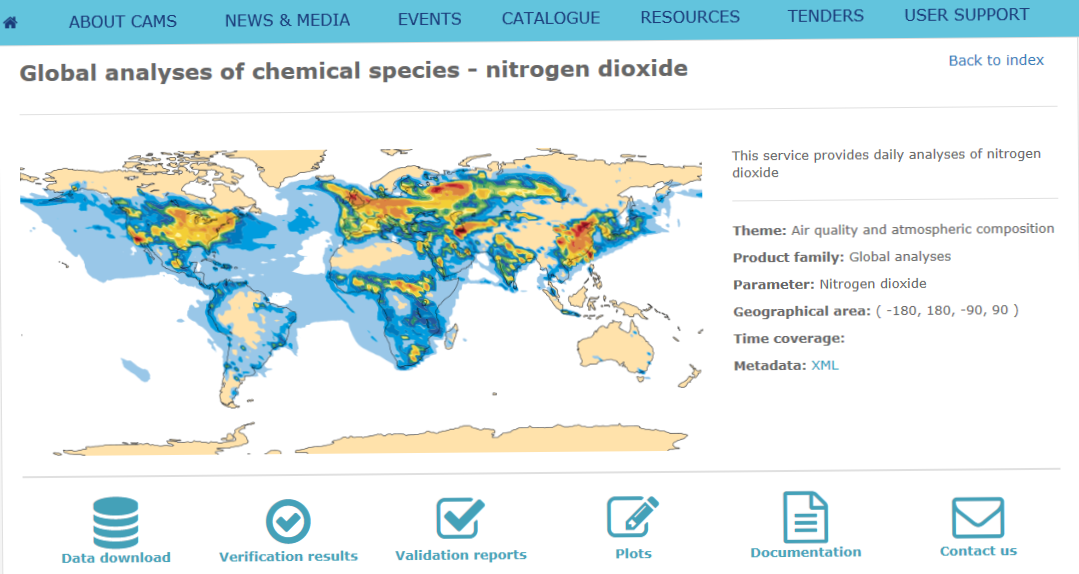
\includegraphics[keepaspectratio=true,width=\dimmin{}{\dimwidth{0.90}}]{images/catalogue}{}\mdline{498}%mdk

%mdk-data-line={499}
\mdhr{}%mdk

%mdk-data-line={500}
\noindent\mdline{500}\mdcaption{\textbf{Figure~\mdcaptionlabel{1}.}~\mdcaptiontext{Available options and details of CAMS Catalogue product ~\emph{Global analyses of chemical species - nitrogen dioxide}}}%mdk
%mdk
\end{mdcenter}\label{cams-catalogue}%mdk
%mdk
\end{figure}%mdk

%mdk-data-line={503}
\noindent\mdline{503}\textbf{For global products}\mdline{503}, \mdline{503}\emph{Plots}\mdline{503} links to a page within CAMS website where an interactive global map is provided. 
Figure\mdline{504}~\mdref{global-map}{\mdcaptionlabel{2}}\mdline{504} shows the generated map of global analysis of NO\mdline{504}\mdsub{2}\mdline{504} concentration for 00:00 UTC December 4th, 2016.
Information about NO\mdline{505}\mdsub{2}\mdline{505} concentration is color-layered on the map with a measurement unit legend provided.
The user is able to adjust the date/time and the vertical area of interest.%mdk

%mdk-data-line={508}
\begin{figure}[h!]%mdk
\begin{mdcenter}%mdk

%mdk-data-line={509}
\noindent\mdline{509}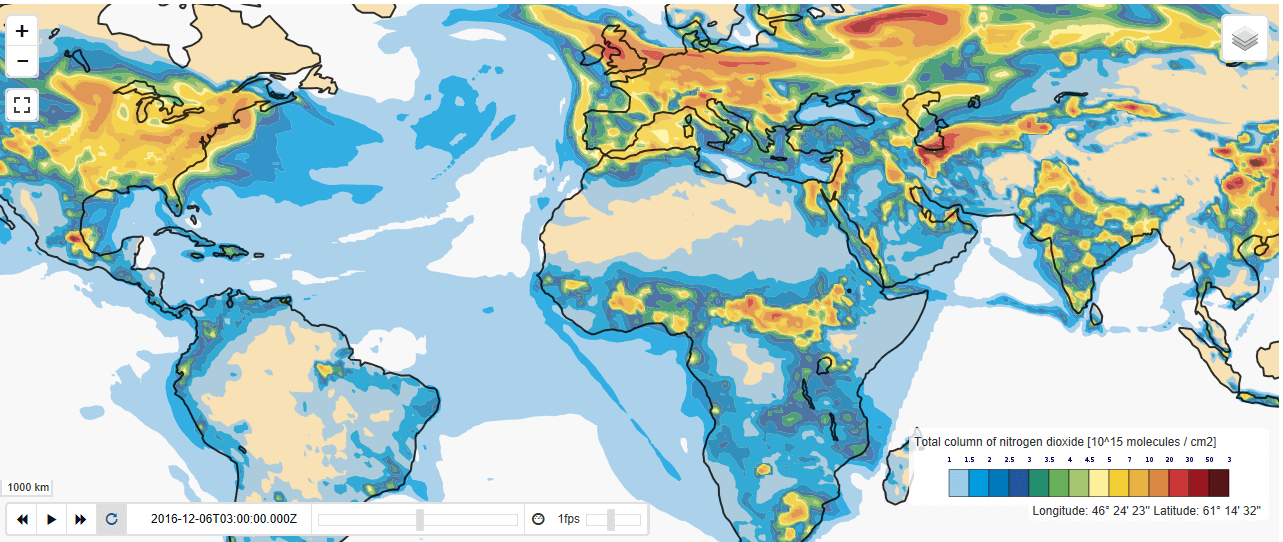
\includegraphics[keepaspectratio=true,width=\dimmin{}{\dimwidth{0.90}}]{images/global_map}{}\mdline{509}%mdk

%mdk-data-line={510}
\mdhr{}%mdk

%mdk-data-line={511}
\noindent\mdline{511}\mdcaption{\textbf{Figure~\mdcaptionlabel{2}.}~\mdcaptiontext{Global analysis of NO\mdsub{2} concentration for December 4th, 2016}}%mdk
%mdk
\end{mdcenter}\label{global-map}%mdk
%mdk
\end{figure}%mdk

%mdk-data-line={513}
\noindent\mdline{513}It should be noted that the plots service seems confusing at first, since both global analyses and forecasts link to the same page.
The distinction between analysis and forecast is based on the date/time selected in respect to current date/time.
Also, the plot service is time-limited in the sense that provides analyses for the past \mdline{515}$5$\mdline{515} days and forecasts for the following \mdline{515}$5$\mdline{515} days only.%mdk

%mdk-data-line={517}
\mdline{517}Global product \mdline{517}\emph{Data download}\mdline{517} link to a page within CAMS website where the user can choose to download data through an interactive interface or through ftp access.
Interactive data access link to ECMWF website. The user is presented a rich web form to select the exact product of interest. This is shown in Figure\mdline{518}~\mdref{global-data}{\mdcaptionlabel{3}}\mdline{518}.
A date-span or specific months can be selected, different vertical levels (surface or pressure dependent or model dependent), multiple time-steps and a huge parameter list, which of course includes NO\mdline{519}\mdsub{2}\mdline{519}.
A drawback is that data for the past four days in respect to current date is not available.%mdk

%mdk-data-line={522}
\begin{figure}[h!]%mdk
\begin{mdcenter}%mdk

%mdk-data-line={523}
\noindent\mdline{523}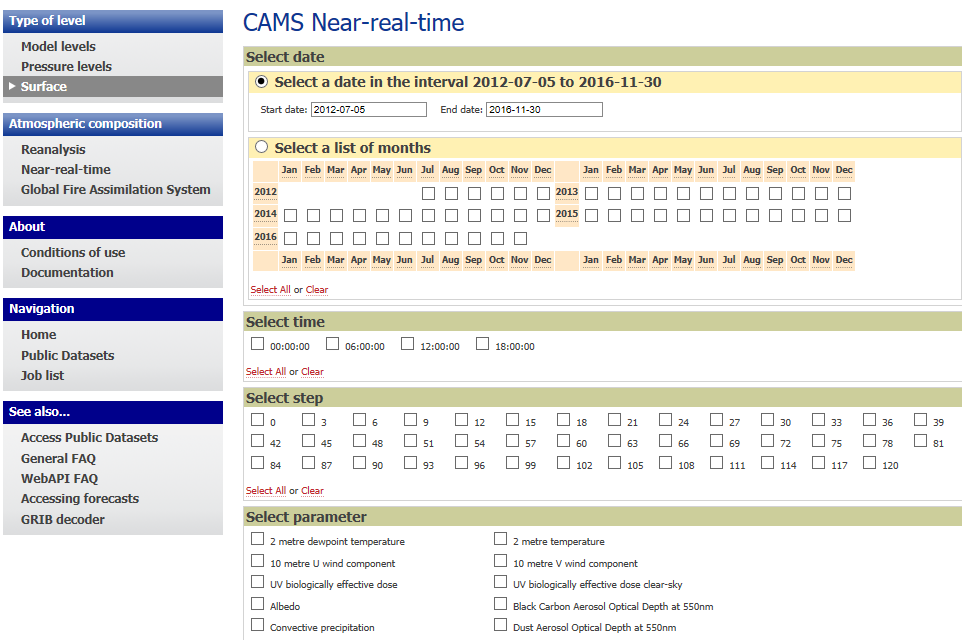
\includegraphics[keepaspectratio=true,width=\dimmin{}{\dimwidth{0.90}}]{images/global_real_time}{}\mdline{523}%mdk

%mdk-data-line={524}
\mdhr{}%mdk

%mdk-data-line={525}
\noindent\mdline{525}\mdcaption{\textbf{Figure~\mdcaptionlabel{3}.}~\mdcaptiontext{User Interface of ECMWF website for downloading data of global analyses and forecasts.}}%mdk
%mdk
\end{mdcenter}\label{global-data}%mdk
%mdk
\end{figure}%mdk

%mdk-data-line={527}
\noindent\mdline{527}After the user has set the filters he is able to download data in both GRID and NetCDF format by clicking the relative link.
In both cases he is led to an \mdline{528}\emph{Additional filtering}\mdline{528} form where he can define the area of interest and the grid resolution as shown in Figure\mdline{528}~\mdref{global-data-additional}{\mdcaptionlabel{4}}\mdline{528}.
The data is then available for downloading.%mdk

%mdk-data-line={531}
\begin{figure}[h!]%mdk
\begin{mdcenter}%mdk

%mdk-data-line={532}
\noindent\mdline{532}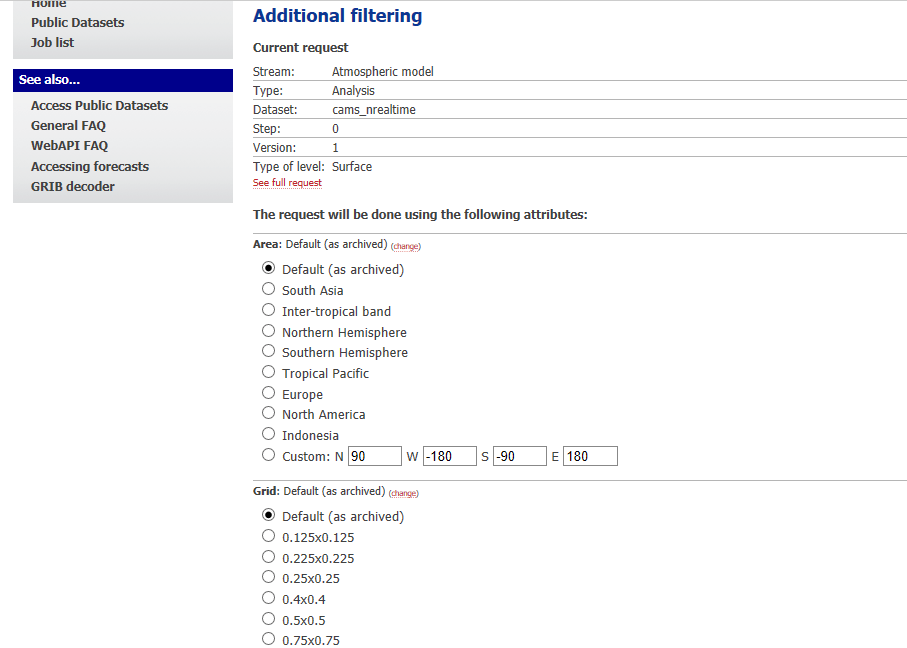
\includegraphics[keepaspectratio=true,width=\dimmin{}{\dimwidth{0.90}}]{images/global_real_time_additional}{}\mdline{532}%mdk

%mdk-data-line={533}
\mdhr{}%mdk

%mdk-data-line={534}
\noindent\mdline{534}\mdcaption{\textbf{Figure~\mdcaptionlabel{4}.}~\mdcaptiontext{Additional filtering of global analyses' and forecasts' data before downloading.}}%mdk
%mdk
\end{mdcenter}\label{global-data-additional}%mdk
%mdk
\end{figure}%mdk

%mdk-data-line={537}
\noindent\mdline{537}\textbf{For regional products}\mdline{537}, both \mdline{537}\emph{Plots}\mdline{537} and \mdline{537}\emph{Data download}\mdline{537} link to the regional subdomain of CAMS website.
The subdomain provides a universal access to individual models and ensemble plots and data for both analyses and forecasts.
This is done by an easy-to-use tab section as seen in Figure.%mdk

%mdk-data-line={541}
\mdline{541}In \mdline{541}\emph{Ensemble Analysis and Forecast}\mdline{541} tab, except from forecasts and analyses maps, additional plots of daily mean and maximum values as well as EPSgrams for 41 major European cities are available (Figure \mdline{541}\#\mdline{541}ensemble-tab).%mdk

%mdk-data-line={543}
\begin{figure}[h!]%mdk
\begin{mdcenter}%mdk

%mdk-data-line={544}
\noindent\mdline{544}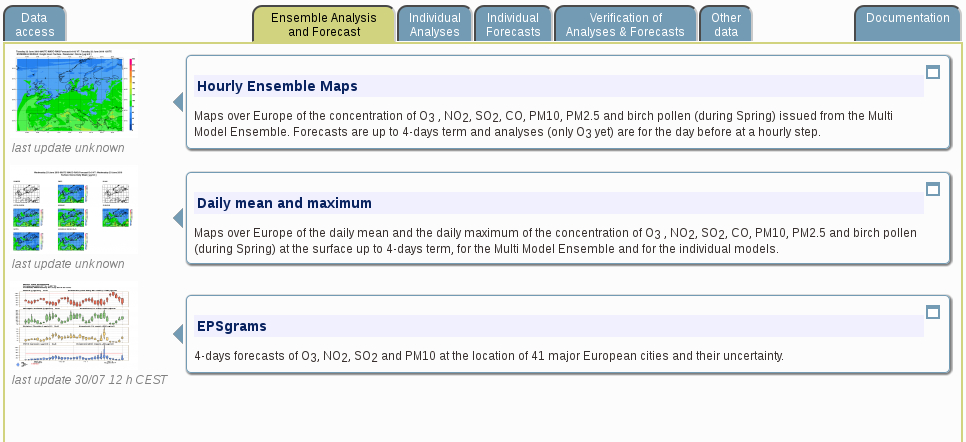
\includegraphics[keepaspectratio=true,width=\dimmin{}{\dimwidth{0.90}}]{images/ensemble_tab}{}\mdline{544}%mdk

%mdk-data-line={545}
\mdhr{}%mdk

%mdk-data-line={546}
\noindent\mdline{546}\mdcaption{\textbf{Figure~\mdcaptionlabel{5}.}~\mdcaptiontext{Available options in \emph{Ensemble Analysis and Forecast} tab}}%mdk
%mdk
\end{mdcenter}\label{ensemble-tab}%mdk
%mdk
\end{figure}%mdk

%mdk-data-line={548}
\noindent\mdline{548}\emph{Hourly Ensemble Maps}\mdline{548} (as well as all maps) provide a friendly user interface (UI) with details of the product, a time navigation bar, filters for base date/time, model, vertical level and parameter options.
The outline is shown in Figure\mdline{549}~\mdref{regional-map-details}{\mdcaptionlabel{6}}\mdline{549}.
\mdline{550}\emph{Hourly Ensemble Maps}\mdline{550} provide analysis and forecasts in the same UI. User first select a base date/time and then, depending on navigation\mdline{550}'\mdline{550}s bar value, he selects forecast or analysis produced on that day.
For example, if selected date/time is 00:00 UTC December 4th, 2016 and time navigation bar value is \mdline{551}$-10$\mdline{551}, then the analysis for 14:00 UTC December 3rd is depicted on the map.
Similarly, given the same date/time and a value of \mdline{552}$+48$\mdline{552} in time navigation bar, the forecast of 00:00 UTC December 6th is shown. 
A useful \mdline{553}\emph{Download PDF}\mdline{553} button, which exports the map to PDF format, is also present.%mdk

%mdk-data-line={555}
\mdline{555}In order to obtain the analysis of NO\mdline{555}\mdsub{2}\mdline{555} concentration on 00:00 UTC December 4th, 2016 we set as date/time the December 5th and a time step of \mdline{555}$-24$\mdline{555}. 
Obtained map is shown in Figure\mdline{556}~\mdref{ensemble-maps}{\mdcaptionlabel{7}}\mdline{556}.%mdk

%mdk-data-line={558}
\begin{figure}[h!]%mdk
\begin{mdcenter}%mdk

%mdk-data-line={559}
\noindent\mdline{559}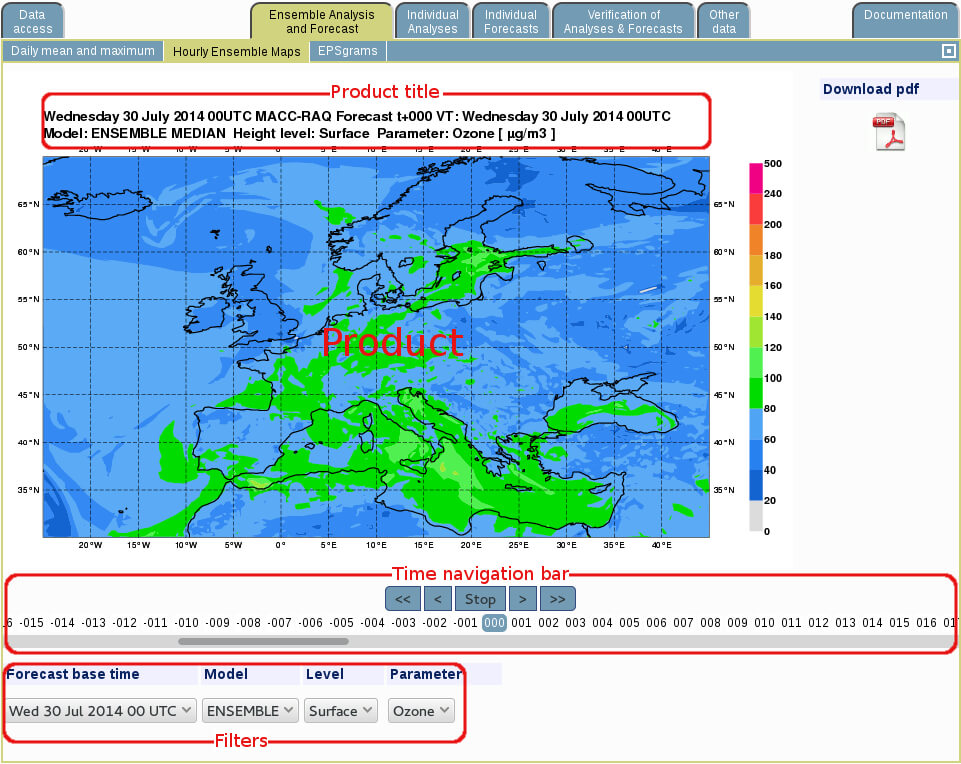
\includegraphics[keepaspectratio=true,width=\dimmin{}{\dimwidth{0.90}}]{images/regional_map_details}{}\mdline{559}%mdk

%mdk-data-line={560}
\mdhr{}%mdk

%mdk-data-line={561}
\noindent\mdline{561}\mdcaption{\textbf{Figure~\mdcaptionlabel{6}.}~\mdcaptiontext{Outline of analyses and forecast maps of regional products.}}%mdk
%mdk
\end{mdcenter}\label{regional-map-details}%mdk
%mdk
\end{figure}%mdk

%mdk-data-line={563}
\begin{figure}[h!]%mdk
\begin{mdcenter}%mdk

%mdk-data-line={564}
\noindent\mdline{564}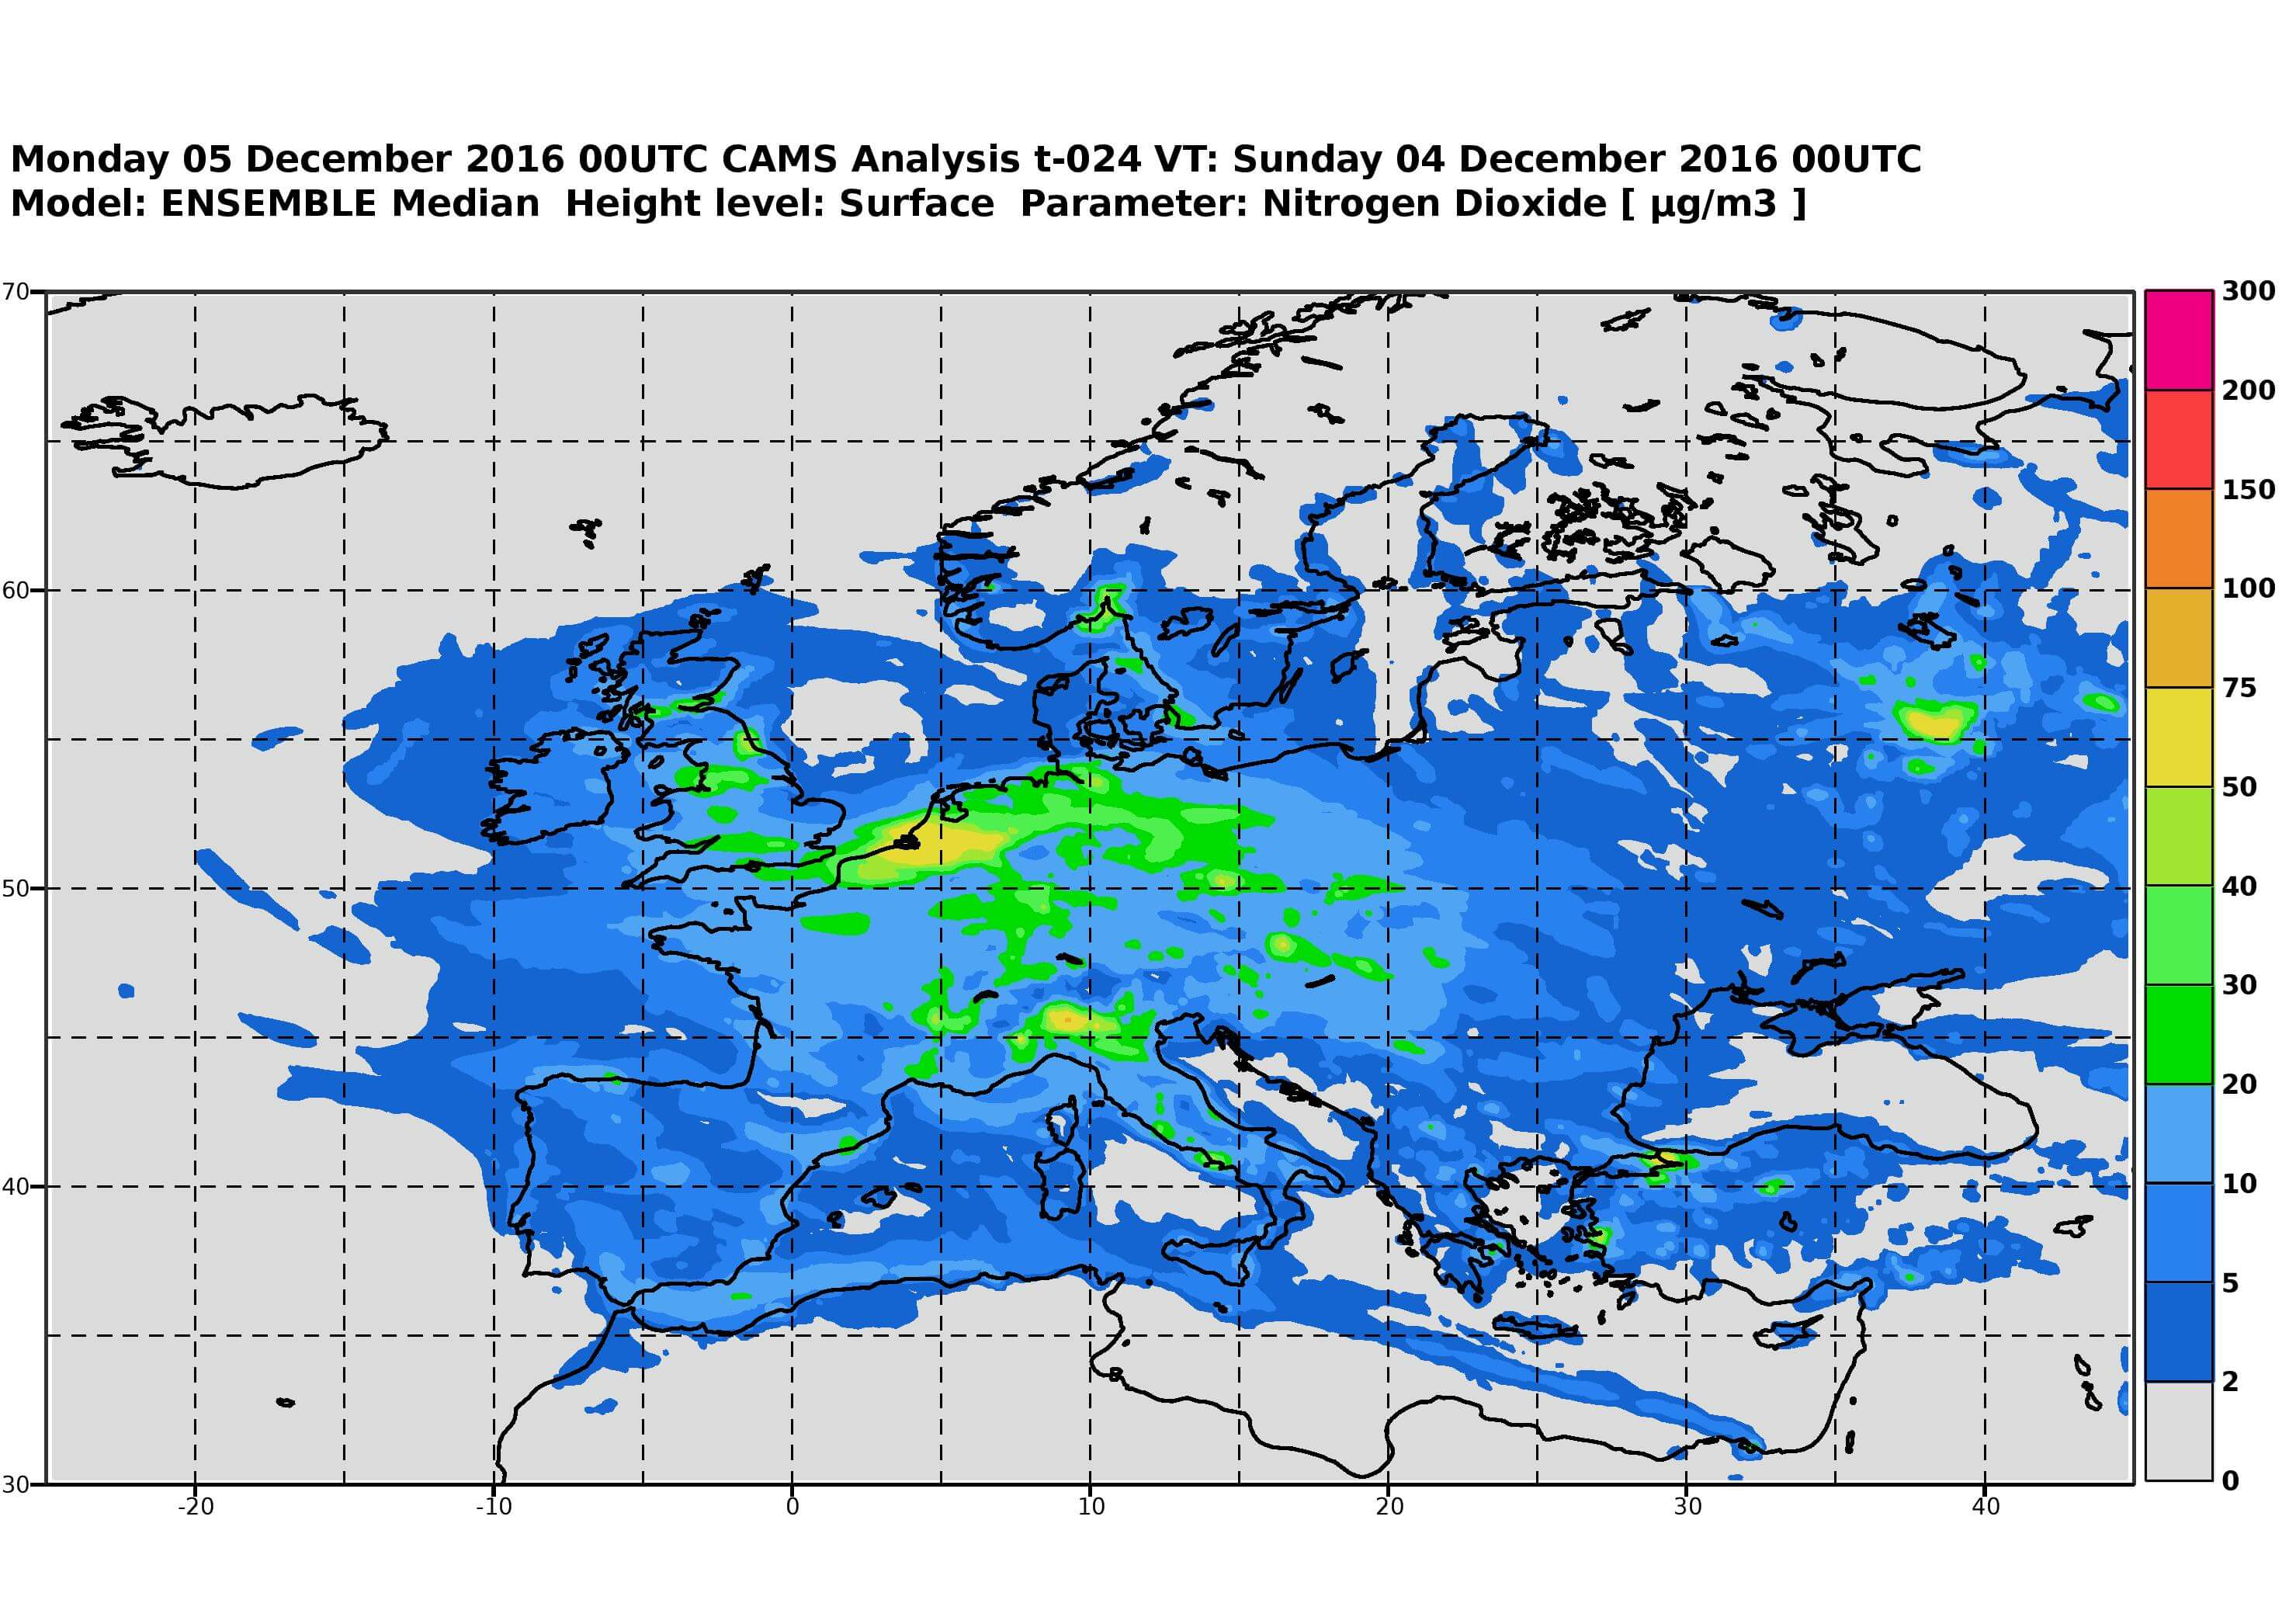
\includegraphics[keepaspectratio=true,width=\dimmin{}{\dimwidth{0.90}}]{images/ensemble_analysis_surface}{}\mdline{564}%mdk

%mdk-data-line={565}
\mdhr{}%mdk

%mdk-data-line={566}
\noindent\mdline{566}\mdcaption{\textbf{Figure~\mdcaptionlabel{7}.}~\mdcaptiontext{Analysis of NO\mdsub{2} concentration on 00:00 UTC December 4th, 2016 issued from the ENSEMBLE model.}}%mdk
%mdk
\end{mdcenter}\label{ensemble-maps}%mdk
%mdk
\end{figure}%mdk

%mdk-data-line={568}
\noindent\mdline{568}\emph{Daily mean and maximum}\mdline{568} tab provides maps of the daily mean and maximum values of the concentration of pollutants as calculated by each model and ensemble.
A useful feature is the ability to view the maps generated of all models side by side. 
This feature is shown in Figure\mdline{570}~\mdref{regional-maximum}{\mdcaptionlabel{8}}\mdline{570} for NO\mdline{570}\mdsub{2}\mdline{570} maximum concentration values on December 4th, 2016.%mdk

%mdk-data-line={572}
\begin{figure}[h!]%mdk
\begin{mdcenter}%mdk

%mdk-data-line={573}
\noindent\mdline{573}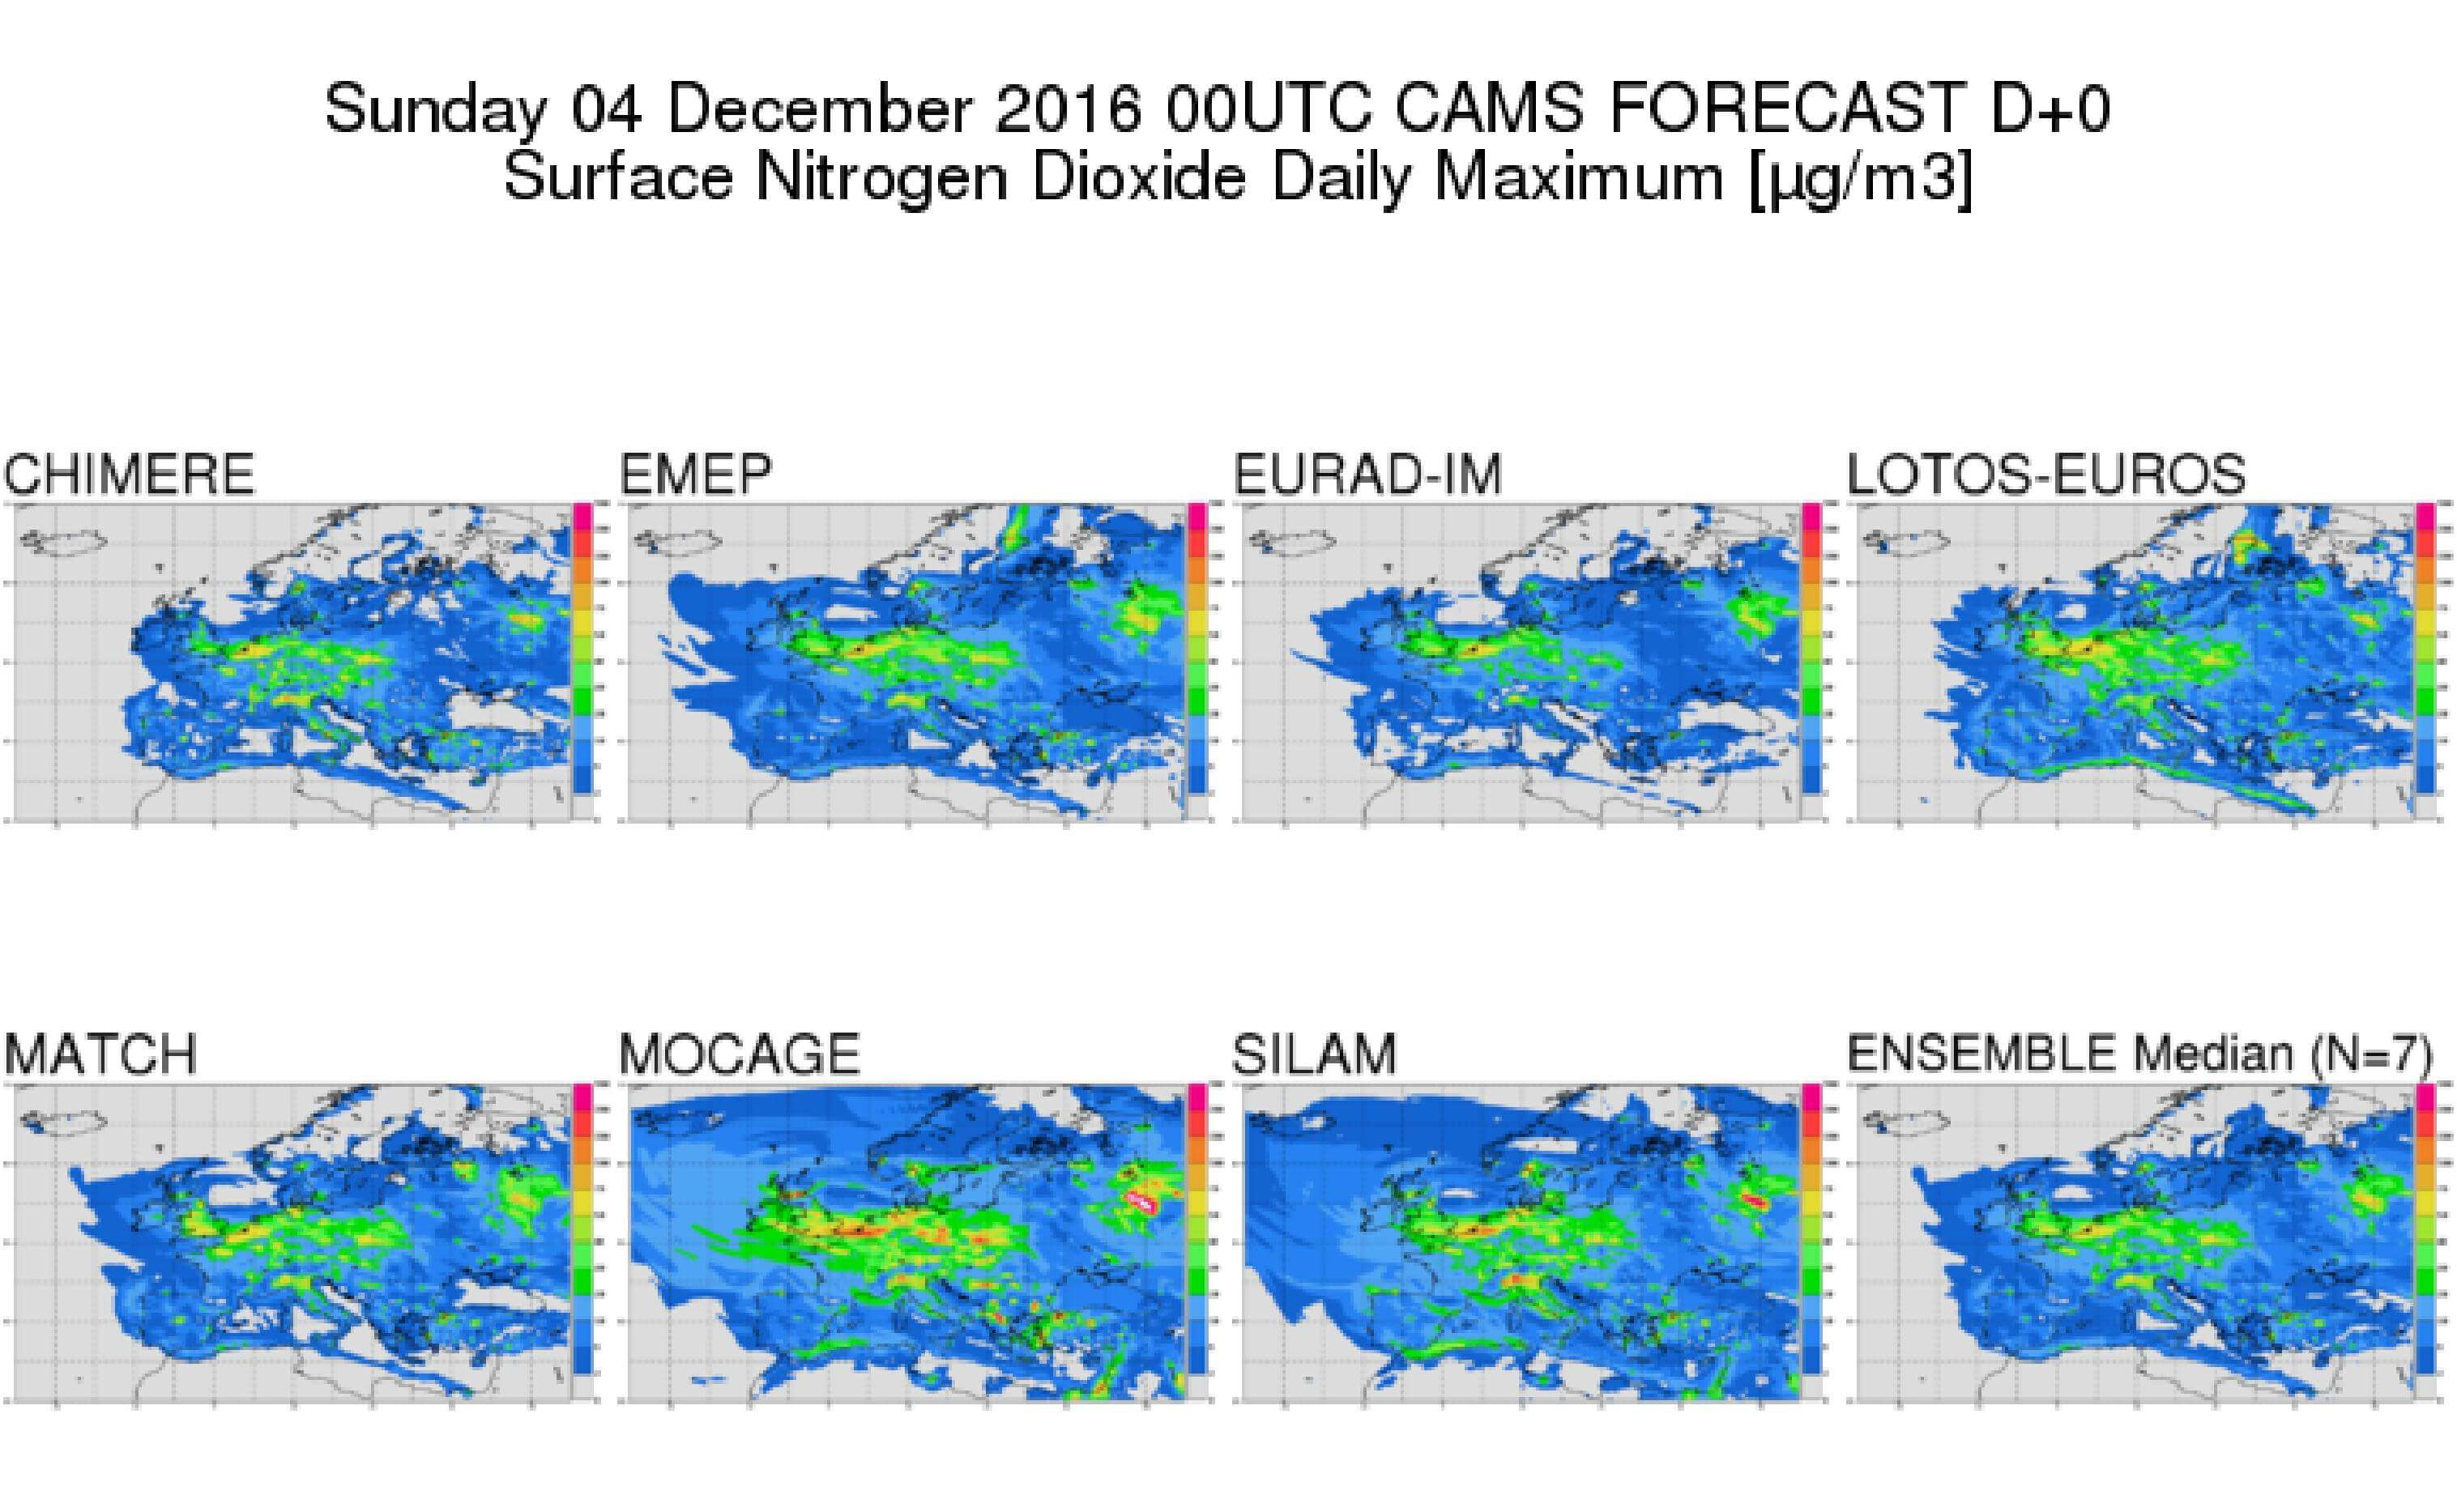
\includegraphics[keepaspectratio=true,width=\dimmin{}{\dimwidth{0.90}}]{images/regional_maximum}{}\mdline{573}%mdk

%mdk-data-line={574}
\mdhr{}%mdk

%mdk-data-line={575}
\noindent\mdline{575}\mdcaption{\textbf{Figure~\mdcaptionlabel{8}.}~\mdcaptiontext{Maximum concentrations of NO\mdsub{2} on December 4th, 2016 as calculated from all models and their ensemble.}}%mdk
%mdk
\end{mdcenter}\label{regional-maximum}%mdk
%mdk
\end{figure}%mdk

%mdk-data-line={577}
\noindent\mdline{577}\emph{EPSgrams}\mdline{577} tab provide 4-days forecasts of O\mdline{577}\mdsub{3}\mdline{577}, NO\mdline{577}\mdsub{2}\mdline{577}, SO\mdline{577}\mdsub{2}\mdline{577} and PM\mdline{577}\mdsub{10}\mdline{577} at the location of 41 major European cities and their uncertainty.
In Figure\mdline{578}~\mdref{regional-epsgram}{\mdcaptionlabel{9}}\mdline{578} forecasts for the city of Athens between December 4th and December 8th, 2016 are shown.%mdk

%mdk-data-line={580}
\begin{figure}[h!]%mdk
\begin{mdcenter}%mdk

%mdk-data-line={581}
\noindent\mdline{581}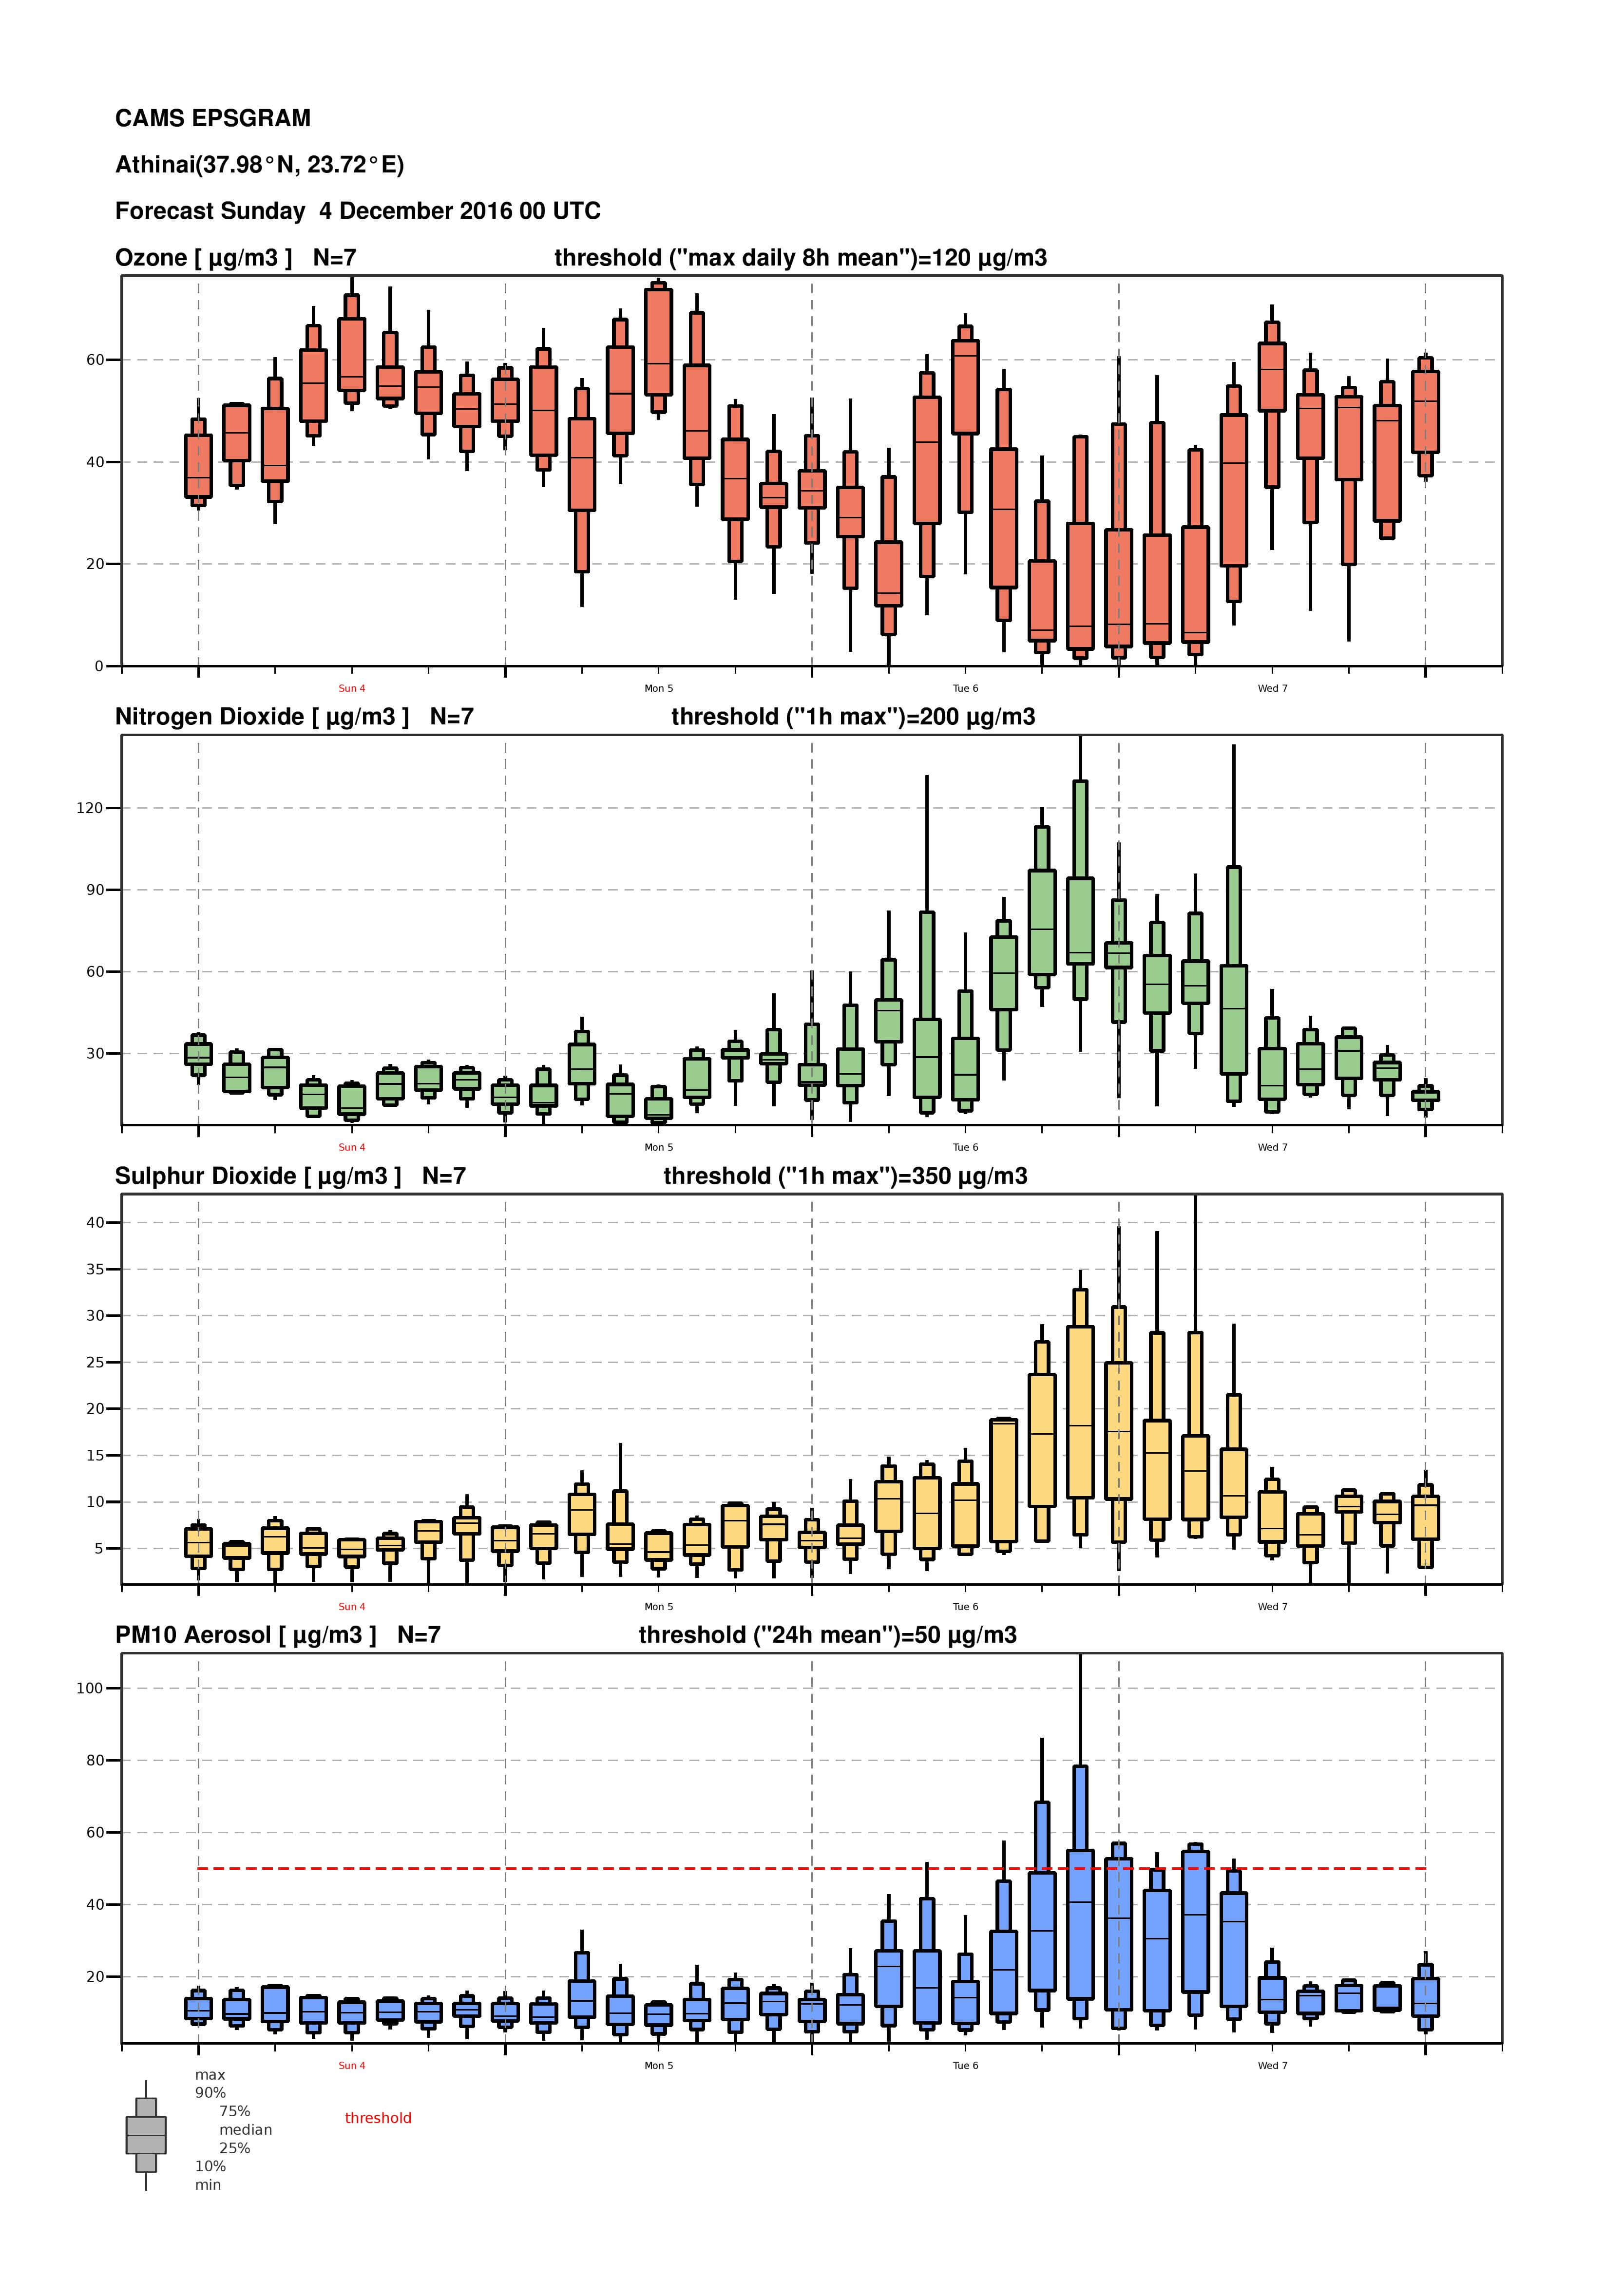
\includegraphics[keepaspectratio=true,width=\dimmin{}{\dimwidth{0.90}}]{images/regional-epsgram}{}\mdline{581}%mdk

%mdk-data-line={582}
\mdhr{}%mdk

%mdk-data-line={583}
\noindent\mdline{583}\mdcaption{\textbf{Figure~\mdcaptionlabel{9}.}~\mdcaptiontext{4-day forecast of O\mdsub{3}, NO\mdsub{2}, SO\mdsub{2} and PM\mdsub{10} at the city of Athens for the period between December 4th - December 8th, 2016.}}%mdk
%mdk
\end{mdcenter}\label{regional-epsgram}%mdk
%mdk
\end{figure}%mdk

%mdk-data-line={586}
\noindent\mdline{586}\emph{Individual Analyses}\mdline{586} and \mdline{586}\emph{Individual Forecasts}\mdline{586} tabs provide maps of pollutants\mdline{586}'\mdline{586} concentration based on individual models calculations.
Analyses are available for the day before at an hourly step. 
Forecasts are available up to 4 days ahead at an hourly step.
It is interesting to see the relevance of the forecast for a given date/time to the post-analysis.
In Figure\mdline{590}~\mdref{chimere-map}{\mdcaptionlabel{10}}\mdline{590} we see the forecast of NO\mdline{590}\mdsub{2}\mdline{590} concentration for December 4th, 2016 issued on December 3rd and the relevant analysis issued on December 5th.
It is obvious that results are quite different.%mdk

%mdk-data-line={593}
\begin{figure}[h!]%mdk
\begin{mdcenter}%mdk
\mdinline{vertical-align=bottom,text-align=center}{\begin{mdtabular}{2}{\dimeval{(\linewidth)/2}}{0pt}%mdk
\begin{tabular}{cc}

%mdk-data-line={595}
\begin{mdcolumn}%mdk
\begin{mdblock}{padding=0.5ex,vertical-align=bottom,text-align=center,width=\dimavailable}%mdk
\mdline{596}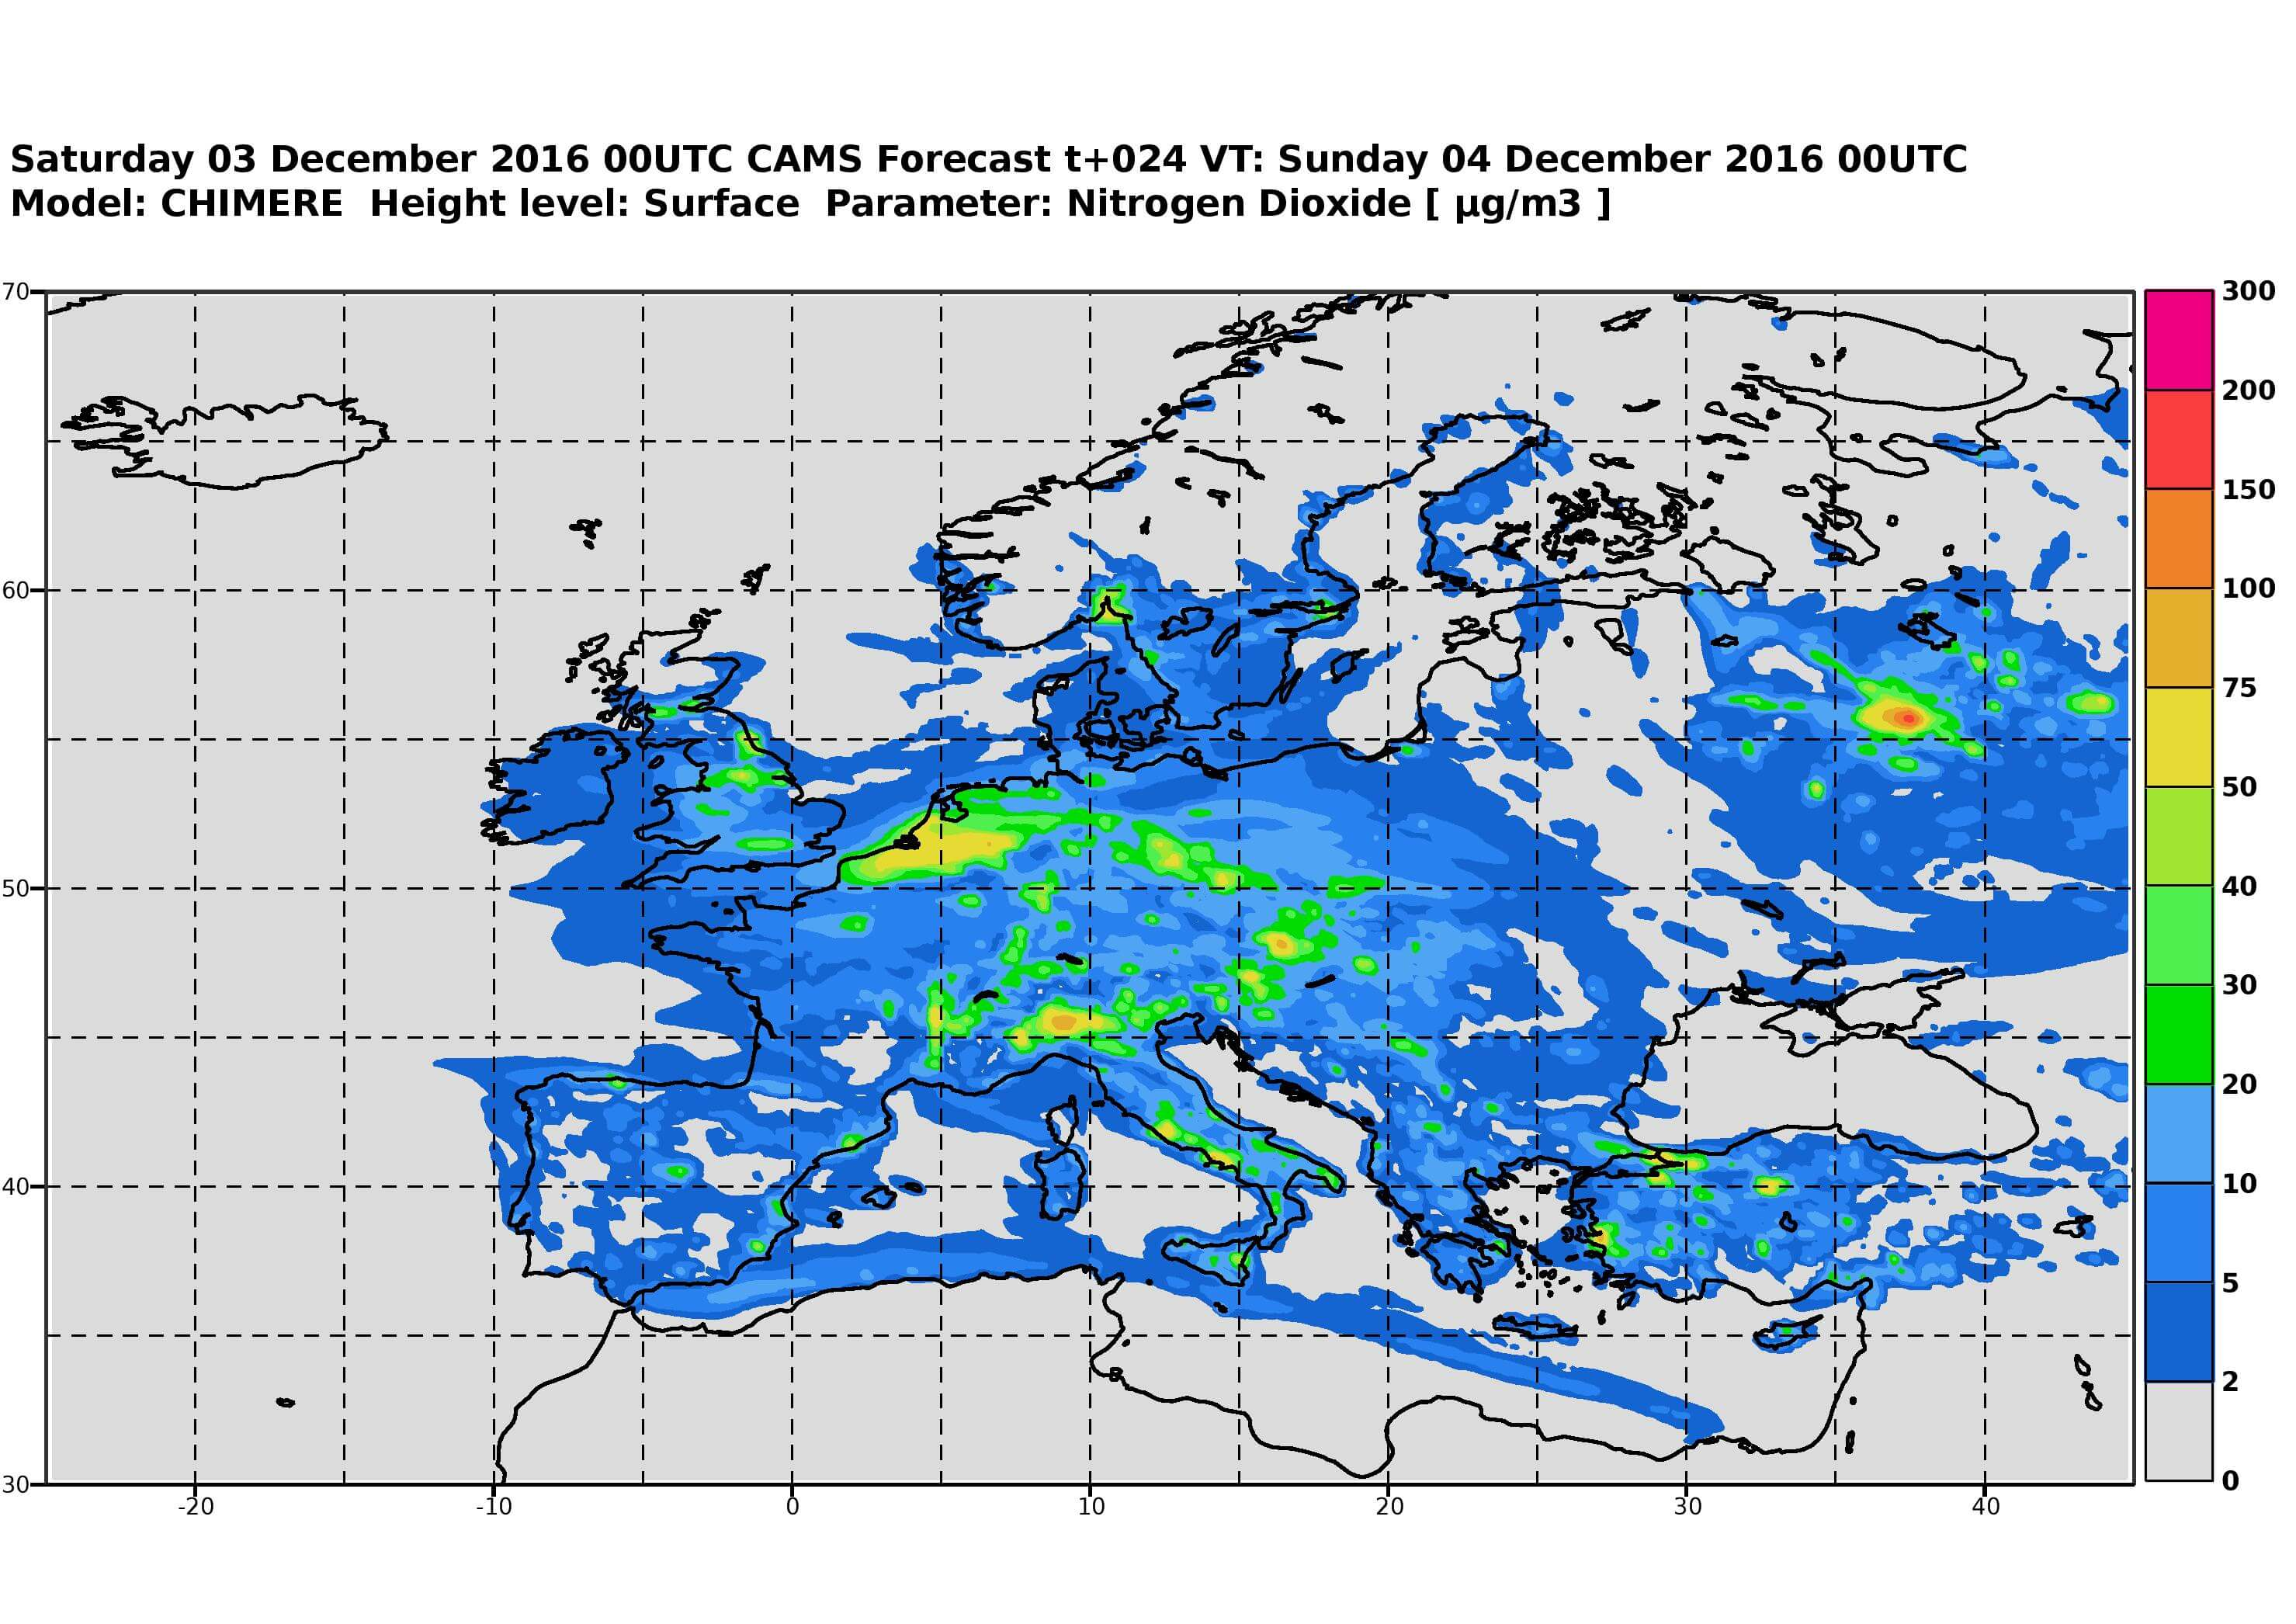
\includegraphics[keepaspectratio=true,width=\dimmin{}{\dimwidth{0.90}}]{images/chimere_forecast}{}\mdline{596}

%mdk-data-line={597}
\begin{mdbmargintb}{1ex}{}%mdk
\mdline{598}(a) \mdline{598} Forecast issued on December 3rd, 2016%mdk
\end{mdbmargintb}%mdk%mdk
\end{mdblock}%mdk
\end{mdcolumn}%mdk
&
%mdk-data-line={598}
\begin{mdcolumn}%mdk
\begin{mdblock}{padding=0.5ex,vertical-align=bottom,text-align=center,width=\dimavailable}%mdk
\mdline{599}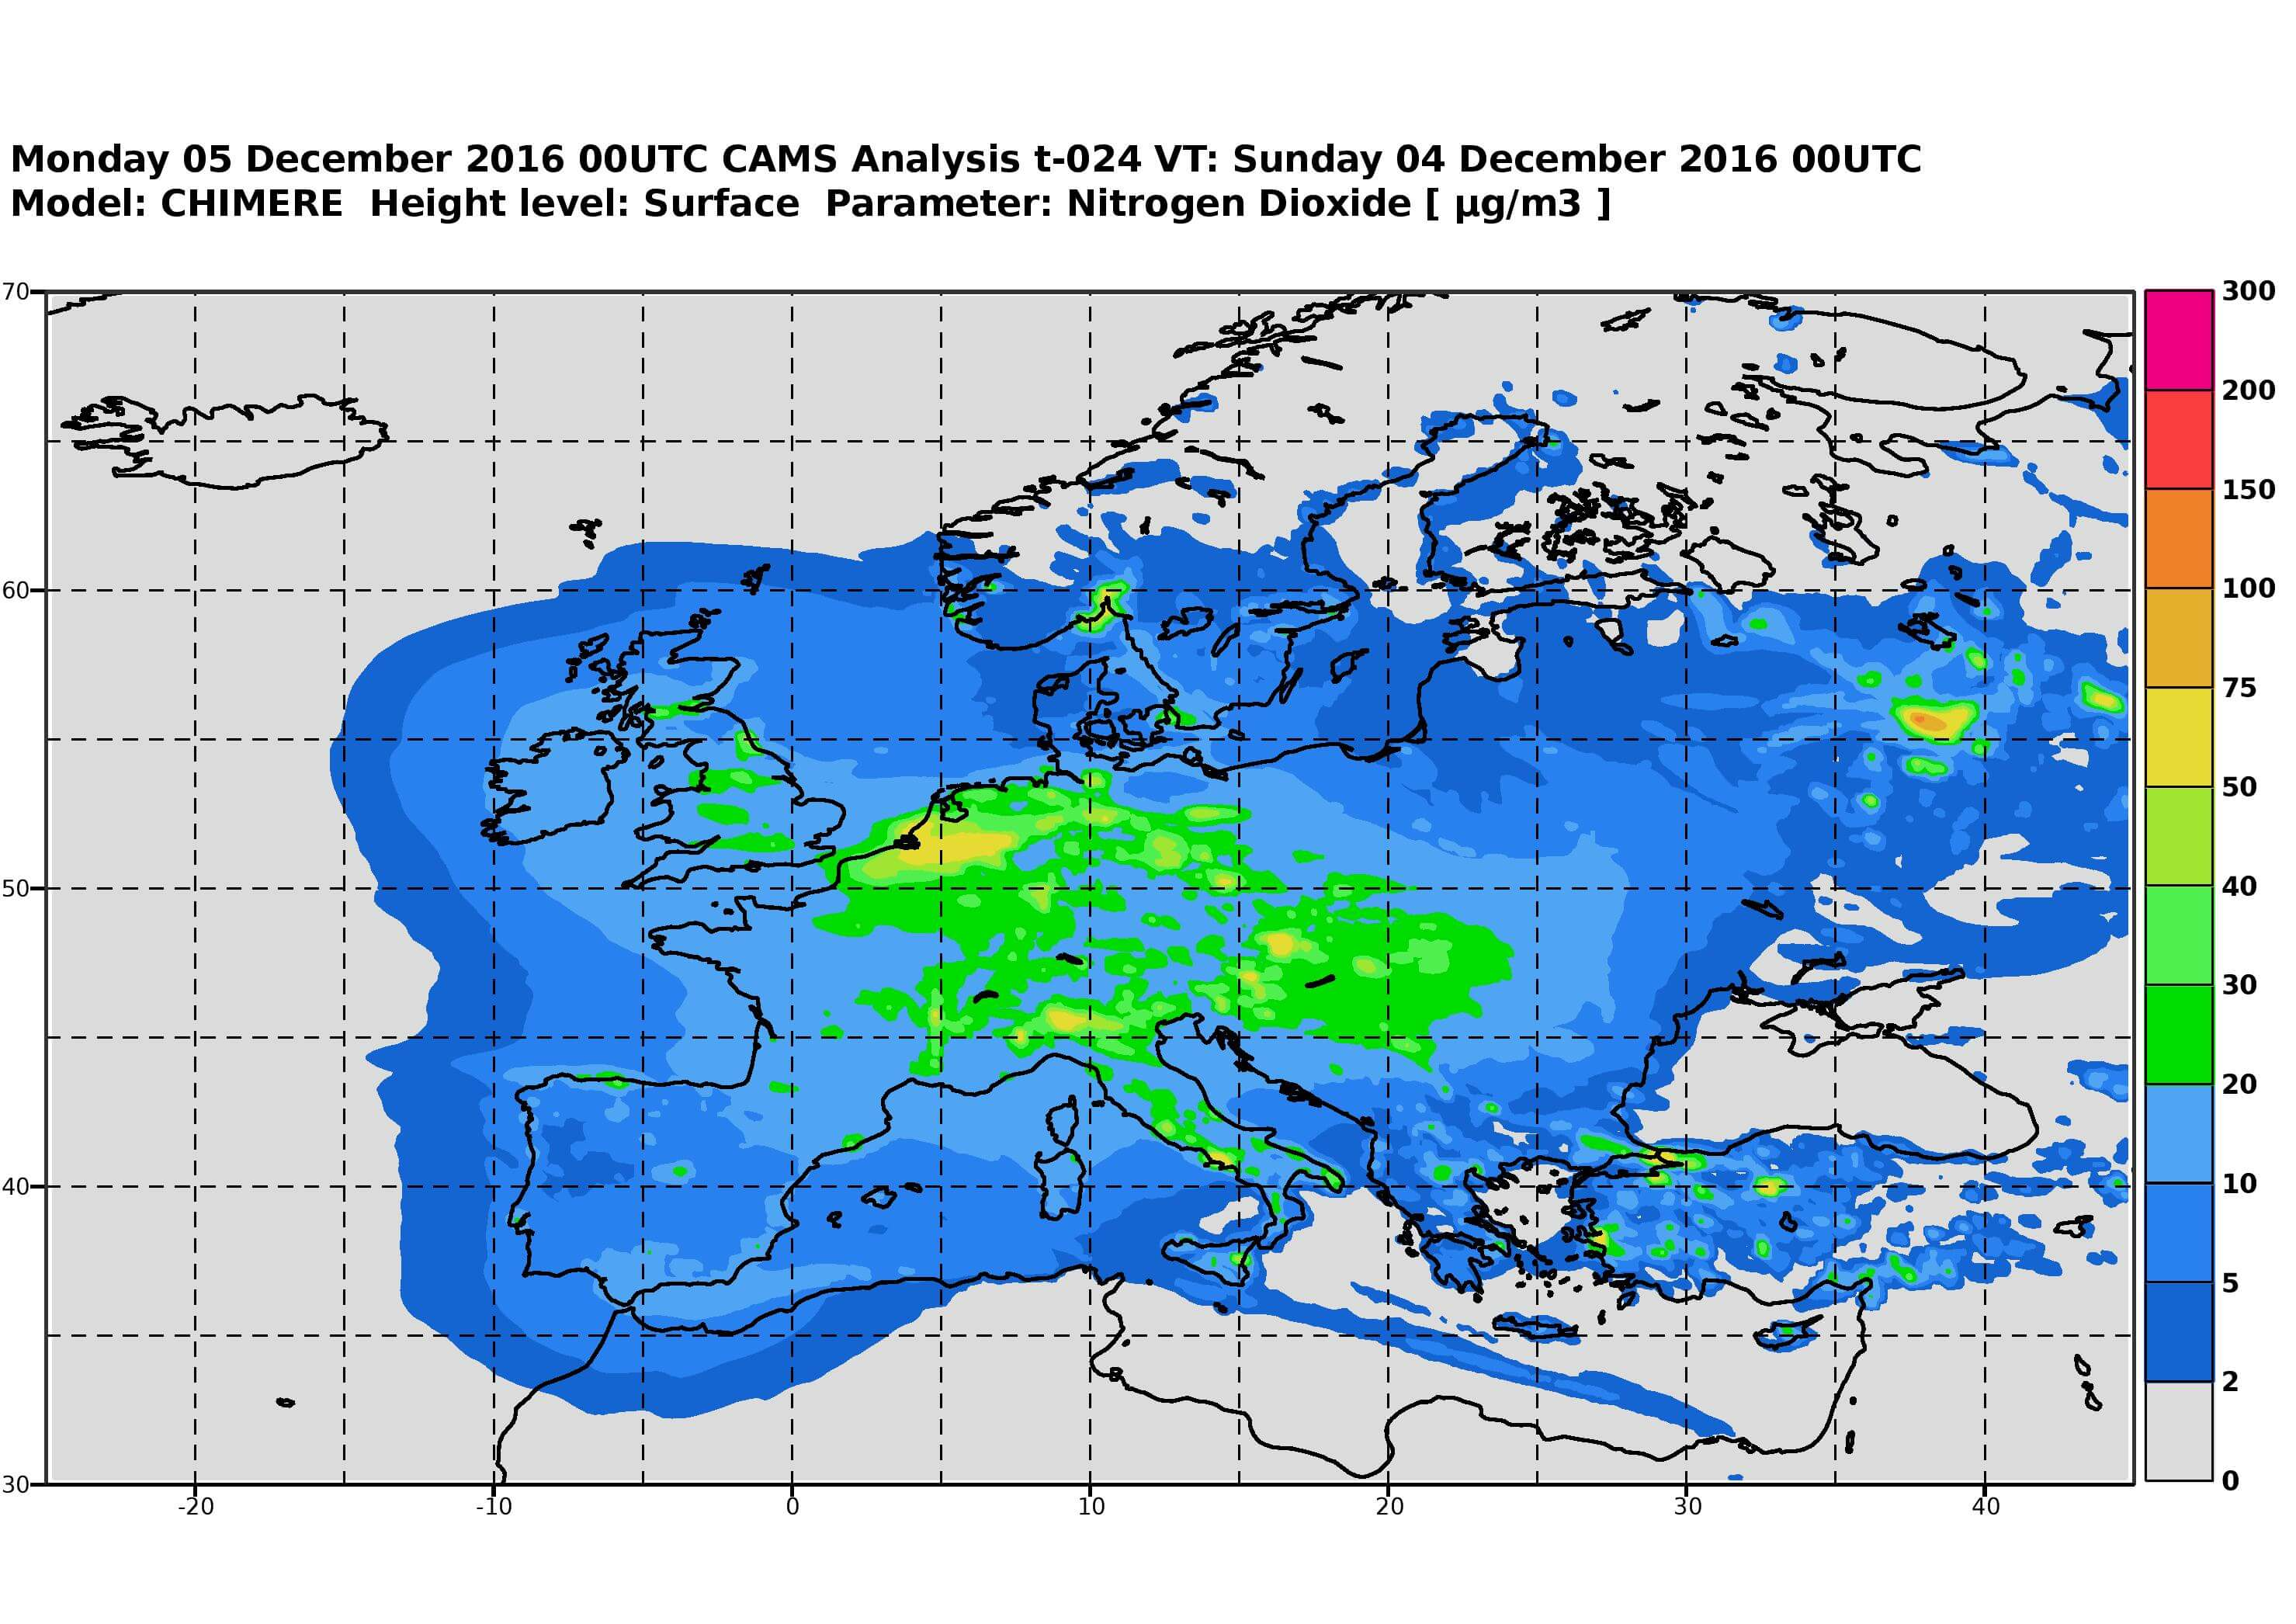
\includegraphics[keepaspectratio=true,width=\dimmin{}{\dimwidth{0.90}}]{images/chimere_analysis}{}\mdline{599}

%mdk-data-line={600}
\begin{mdbmargintb}{1ex}{}%mdk
\mdline{601}(b) \mdline{601} Analysis issued on December 5th, 2016%mdk
\end{mdbmargintb}%mdk%mdk
\end{mdblock}%mdk
\end{mdcolumn}%mdk
\\
\end{tabular}\end{mdtabular}
}
%mdk-data-line={602}
\mdhr{}%mdk

%mdk-data-line={603}
\noindent\mdline{603}\mdcaption{\textbf{Figure~\mdcaptionlabel{10}.}~\mdcaptiontext{Forecast and analysis maps of NO\mdsub{2} concentration for December 4th, 2016 issued by the CHIMERE model.}}%mdk
%mdk
\end{mdcenter}\label{chimere-map}%mdk
%mdk
\end{figure}%mdk

%mdk-data-line={608}
\noindent\mdline{608}Data files are very easy to download. Under the filters section there is a \mdline{608}\emph{Direct Data Access}\mdline{608} section with a checkbox for accepting the CAMS data licence.
Once the checkbox is checked we are presented with the details of the product (model, pollutant, base date/time) and an optional selectbox with available options depending on the product.
After an option is selected a direct download in NetCDF format is available by clicking the button.%mdk

%mdk-data-line={612}
\section{\mdline{612}5.\hspace*{0.5em}\mdline{612}Conclusions}\label{sec-conclusions}%mdk%mdk

%mdk-data-line={614;out/technical_report-bib.bbl.mdk:1}
%mdk-data-line={614;out/technical_report-bib.bbl.mdk:2}
\mdsetrefname{References}%mdk
{\mdsupressbiblabel\mdbibindent{2}\begin{thebibliography}{28}%mdk
\label{sec-bibliography}%mdk

%mdk-data-line={bibliography.bib:75}
\bibitem{annamalai2007combustion}\mdbibitemlabel{}Annamalai, K.~(2007), \emph{Combustion science and engineering}, CRC Press/Taylor \& Francis, Boca Raton.\label{annamalai2007combustion}%mdk%mdk

%mdk-data-line={bibliography.bib:99}
\bibitem{beekmann2010modelling}\mdbibitemlabel{}Beekmann, M., and R.~Vautard (2010), A modelling study of photochemical regimes over Europe: robustness and variability, \emph{Atmos. Chem. Phys}, \emph{10}, 10067–10084.\label{beekmann2010modelling}%mdk%mdk

%mdk-data-line={bibliography.bib:26}
\bibitem{bell2006exposure}\mdbibitemlabel{}Bell, M.~L., R.~D.~Peng, and F.~Dominici (2006), The exposure-response curve for ozone and risk of mortality and the adequacy of current ozone regulations, \emph{Environmental health perspectives}, 532–536.\label{bell2006exposure}%mdk%mdk

%mdk-data-line={bibliography.bib:283}
\bibitem{bousserez2007evaluation}\mdbibitemlabel{}Bousserez, N.~et al. (2007), Evaluation of the MOCAGE chemistry transport model during the ICARTT/ITOP experiment, \emph{Journal of Geophysical Research: Atmospheres}, \emph{112}(D10).\label{bousserez2007evaluation}%mdk%mdk

%mdk-data-line={bibliography.bib:85}
\bibitem{epabulletin}\mdbibitemlabel{}Clean Air Technology Center, I.~Transfer, P.~I.~Division, O.~of Air Quality Planning, Standards, U.~S.~E.~P.~Agency, and N.~C.~Research Triangle Park (1999), \emph{Nitrogen Oxides, why and how they are controlled}.\label{epabulletin}%mdk%mdk

%mdk-data-line={bibliography.bib:119}
\bibitem{colette2011air}\mdbibitemlabel{}Colette, A.~et al. (2011), Air quality trends in Europe over the past decade: a first multi-model assessment, \emph{Atmospheric Chemistry and Physics}, \emph{11}(22), 11657–11678.\label{colette2011air}%mdk%mdk

%mdk-data-line={bibliography.bib:240}
\bibitem{curier2012improving}\mdbibitemlabel{}Curier, R., R.~Timmermans, S.~Calabretta-Jongen, H.~Eskes, A.~Segers, D.~Swart, and M.~Schaap (2012), Improving ozone forecasts over Europe by synergistic use of the LOTOS-EUROS chemical transport model and in-situ measurements, \emph{Atmospheric environment}, \emph{60}, 217–226.\label{curier2012improving}%mdk%mdk

%mdk-data-line={bibliography.bib:148}
\bibitem{fagerli2008trends}\mdbibitemlabel{}Fagerli, H., and W.~Aas (2008), Trends of nitrogen in air and precipitation: Model results and observations at EMEP sites in Europe, 1980\textendash{}2003, \emph{Environmental Pollution}, \emph{154}(3), 448–461.\label{fagerli2008trends}%mdk%mdk

%mdk-data-line={bibliography.bib:1}
\bibitem{forster2007changes}\mdbibitemlabel{}Forster, P.~et al. (2007), Changes in atmospheric constituents and in radiative forcing. Chapter 2, in \emph{Climate Change 2007. The Physical Science Basis}.\label{forster2007changes}%mdk%mdk

%mdk-data-line={bibliography.bib:35}
\bibitem{fowler2008ground}\mdbibitemlabel{}Fowler, D.~et al. (2008), Ground-level ozone in the 21st century: future trends, impacts and policy implications, \emph{Royal Society Science Policy Report}, \emph{15}(08).\label{fowler2008ground}%mdk%mdk

%mdk-data-line={bibliography.bib:159}
\bibitem{genberg2013light}\mdbibitemlabel{}Genberg, J.~et al. (2013), Light-absorbing carbon in Europe\textendash{}measurement and modelling, with a focus on residential wood combustion emissions, \emph{Atmospheric Chemistry and Physics}, \emph{13}(17), 8719–8738.\label{genberg2013light}%mdk%mdk

%mdk-data-line={bibliography.bib:141}
\bibitem{jonson2006first}\mdbibitemlabel{}Jonson, J., P.~Wind, M.~Gauss, S.~Tsyro, A.~S\o{}vde, H.~Klein, I.~Isaksen, and L.~Tarras\'{o}n (2006), First results from the hemispheric EMEP model and comparison with the global Oslo CTM2 model, \emph{The Norwegian Meteorological Institute, Oslo, Norway}.\label{jonson2006first}%mdk%mdk

%mdk-data-line={bibliography.bib:272}
\bibitem{josse2004radon}\mdbibitemlabel{}Josse, B., P.~Simon, and V.-H.~Peuch (2004), Radon global simulations with the multiscale chemistry and transport model MOCAGE, \emph{Tellus B}, \emph{56}(4), 339–356.\label{josse2004radon}%mdk%mdk

%mdk-data-line={bibliography.bib:293}
\bibitem{lacressonniere2014european}\mdbibitemlabel{}Lacressonni\`{e}re, G., V.-H.~Peuch, R.~Vautard, J.~Arteta, M.~D\'{e}qu\'{e}, M.~Joly, B.~Josse, V.~Mar\'{e}cal, and D.~Saint-Martin (2014), European air quality in the 2030s and 2050s: impacts of global and regional emission trends and of climate change, \emph{Atmospheric Environment}, \emph{92}, 348–358.\label{lacressonniere2014european}%mdk%mdk

%mdk-data-line={bibliography.bib:261}
\bibitem{langner1998validation}\mdbibitemlabel{}Langner, J., L.~Robertson, C.~Persson, and A.~Ullerstig (1998), Validation of the operational emergency response model at the Swedish meteorological and hydrological institute using data from ETEX and the Chernobyl accident, \emph{Atmospheric Environment}, \emph{32}(24), 4325–4333.\label{langner1998validation}%mdk%mdk

%mdk-data-line={bibliography.bib:92}
\bibitem{menut2013chimere}\mdbibitemlabel{}Menut, L.~et al. (2013), CHIMERE 2013: a model for regional atmospheric composition modelling, Geosci. Model Dev., 6, 981\textendash{}1028, doi: 10.5194,\label{menut2013chimere}%mdk%mdk

%mdk-data-line={bibliography.bib:55}
\bibitem{mollenhauer2010handbook}\mdbibitemlabel{}Mollenhauer, K., and H.~Tschöke (2010), \emph{Handbook of diesel engines}, Springer.\label{mollenhauer2010handbook}%mdk%mdk

%mdk-data-line={bibliography.bib:200}
\bibitem{monteiro2013bias}\mdbibitemlabel{}Monteiro, A.~et al. (2013), Bias correction techniques to improve air quality ensemble predictions: focus on O3 and PM over Portugal, \emph{Environmental Modeling \& Assessment}, \emph{18}(5), 533–546.\label{monteiro2013bias}%mdk%mdk

%mdk-data-line={bibliography.bib:63}
\bibitem{omidvarborna2015113}\mdbibitemlabel{}Omidvarborna, H., A.~Kumar, and D.-S.~Kim (2015), NOx emissions from low-temperature combustion of biodiesel made of various feedstocks and blends, \emph{Fuel Processing Technology}, \emph{140}, 113 – 118, doi:\href{https://dx.doi.org/10.1016/j.fuproc.2015.08.031}{10.1016/j.fuproc.2015.08.031}.\label{omidvarborna2015113}%mdk%mdk

%mdk-data-line={bibliography.bib:211}
\bibitem{paschalidi2015inverse}\mdbibitemlabel{}Paschalidi, Z.~(2015), Inverse modelling for the tropospheric chemical state estimation by 4-dimensional variational data assimilation from routinely and campaign platforms, phdthesis, Universit\"{a}t zu K\"{o}ln.\label{paschalidi2015inverse}%mdk%mdk

%mdk-data-line={bibliography.bib:303}
\bibitem{rouil2009prev}\mdbibitemlabel{}Rouil, L.~et al. (2009), PREV’AIR, \emph{Bulletin of the American Meteorological Society}, \emph{90}(1), 73.\label{rouil2009prev}%mdk%mdk

%mdk-data-line={bibliography.bib:8}
\bibitem{sabziparvar1998changes}\mdbibitemlabel{}Sabziparvar, A.~A., D.~F.~Forster, and K.~P.~Shine (1998), Changes in ultraviolet radiation due to stratospheric and tropospheric ozone changes since preindustrial times, \emph{Journal of geophysical research}, \emph{103}(D20), 26107–26113.\label{sabziparvar1998changes}%mdk%mdk

%mdk-data-line={bibliography.bib:218}
\bibitem{schaap2008lotos}\mdbibitemlabel{}Schaap, M., R.~M.~Timmermans, M.~Roemer, G.~Boersen, P.~Builtjes, F.~Sauter, G.~Velders, and J.~Beck (2008), The LOTOS-EUROS model: description, validation and latest developments, \emph{International Journal of Environment and Pollution}, \emph{32}(2), 270–290.\label{schaap2008lotos}%mdk%mdk

%mdk-data-line={bibliography.bib:18}
\bibitem{seinfeld2006atmospheric}\mdbibitemlabel{}Seinfeld, J.~H., and S.~N.~Pandis (2006), \emph{Atmospheric chemistry and physics. Hoboken}, NJ: Wiley.\label{seinfeld2006atmospheric}%mdk%mdk

%mdk-data-line={bibliography.bib:44}
\bibitem{sitch2007indirect}\mdbibitemlabel{}Sitch, S., P.~Cox, W.~Collins, and C.~Huntingford (2007), Indirect radiative forcing of climate change through ozone effects on the land-carbon sink, \emph{Nature}, \emph{448}(7155), 791–794.\label{sitch2007indirect}%mdk%mdk

%mdk-data-line={bibliography.bib:314}
\bibitem{sofiev2008construction}\mdbibitemlabel{}Sofiev, M., M.~Galperin, and E.~Genikhovich (2008), A construction and evaluation of Eulerian dynamic core for the air quality and emergency modelling system SILAM, in \emph{Air Pollution Modeling and Its Application XIX}, pp. 699–701, Springer.\label{sofiev2008construction}%mdk%mdk

%mdk-data-line={bibliography.bib:250}
\bibitem{vlemmix2015max}\mdbibitemlabel{}Vlemmix, T., H.~Eskes, A.~Piters, M.~Schaap, F.~Sauter, H.~Kelder, and P.~Levelt (2015), MAX-DOAS tropospheric nitrogen dioxide column measurements compared with the Lotos-Euros air quality model, \emph{Atmospheric Chemistry and Physics}, \emph{15}(3), 1313–1330.\label{vlemmix2015max}%mdk%mdk

%mdk-data-line={bibliography.bib:229}
\bibitem{de2011six}\mdbibitemlabel{}Wildt, M.~de R.~de, H.~Eskes, A.~Manders, F.~Sauter, M.~Schaap, D.~Swart, and P.~van Velthoven (2011), Six-day PM 10 air quality forecasts for the Netherlands with the chemistry transport model Lotos-Euros, \emph{Atmospheric environment}, \emph{45}(31), 5586–5594.\label{de2011six}%mdk%mdk
\par%mdk
\end{thebibliography}}%mdk%mdk%mdk


\end{document}
